\documentclass[11pt]{article}

% ----------------------------
% Packages
% ----------------------------
\usepackage[margin=1in]{geometry}
\usepackage{amsmath, amssymb}
\usepackage{graphicx}
\usepackage{movie15}
\usepackage{booktabs}
\usepackage{siunitx}
\usepackage{physics}
\usepackage{hyperref}
\usepackage{caption}
\usepackage{subcaption}
\usepackage{hyperref}
\usepackage[round]{natbib}



% ----------------------------
% Title Information
% ----------------------------
\title{A Multiscale Modeling Framework for Contrail Formation and Persistence
Using Plume-Scale Simulations and Reanalysis Meteorology}

\author{Shriman Jha}
\date{\today}

% ----------------------------
\begin{document}
\maketitle

% ----------------------------

% ----------------------------
\section{Introduction}

\subsection{Contrails and Radiative Forcing}

Aircraft condensation trails (contrails) are line-shaped ice clouds that form in the
upper troposphere when moist aircraft exhaust mixes with cold ambient air and becomes
supersaturated with respect to ice \cite{Schumann1996,Schumann2017Monograph}.
Under favorable atmospheric conditions, contrails can persist for hours and spread into
cirrus-like cloud decks (contrail cirrus), exerting a net warming influence on Earth’s climate
\cite{BurkhardtKarcher2011,Karcher2018,Lee2021}.
Unlike low-level clouds, which primarily affect shortwave radiation, contrails typically form at high
altitudes where temperatures are substantially lower than at the surface, making their longwave
radiative impact dominant \cite{Karcher2018,Lee2021}.


The physical basis for this effect follows directly from the Stefan--Boltzmann law,
\begin{equation}
    F = \sigma T^4,
\end{equation}
which governs thermal emission from a body at temperature $T$. Because emission scales
strongly with temperature, radiation emitted from cold upper-tropospheric cloud layers
is substantially weaker than radiation emitted from the warm surface and lower
troposphere.

Figure~\ref{fig:contrail_radiation} illustrates this mechanism schematically. A contrail
forming near the tropopause acts as a radiatively cold layer overlying a much warmer
atmosphere below. Longwave radiation emitted to space is therefore characteristic of the
contrail temperature rather than the surface temperature, leading to a reduction in outgoing longwave radiation and a positive radiative forcing
\cite{BurkhardtKarcher2011,Karcher2018,Lee2021}.

\begin{figure}[t]
    \centering
    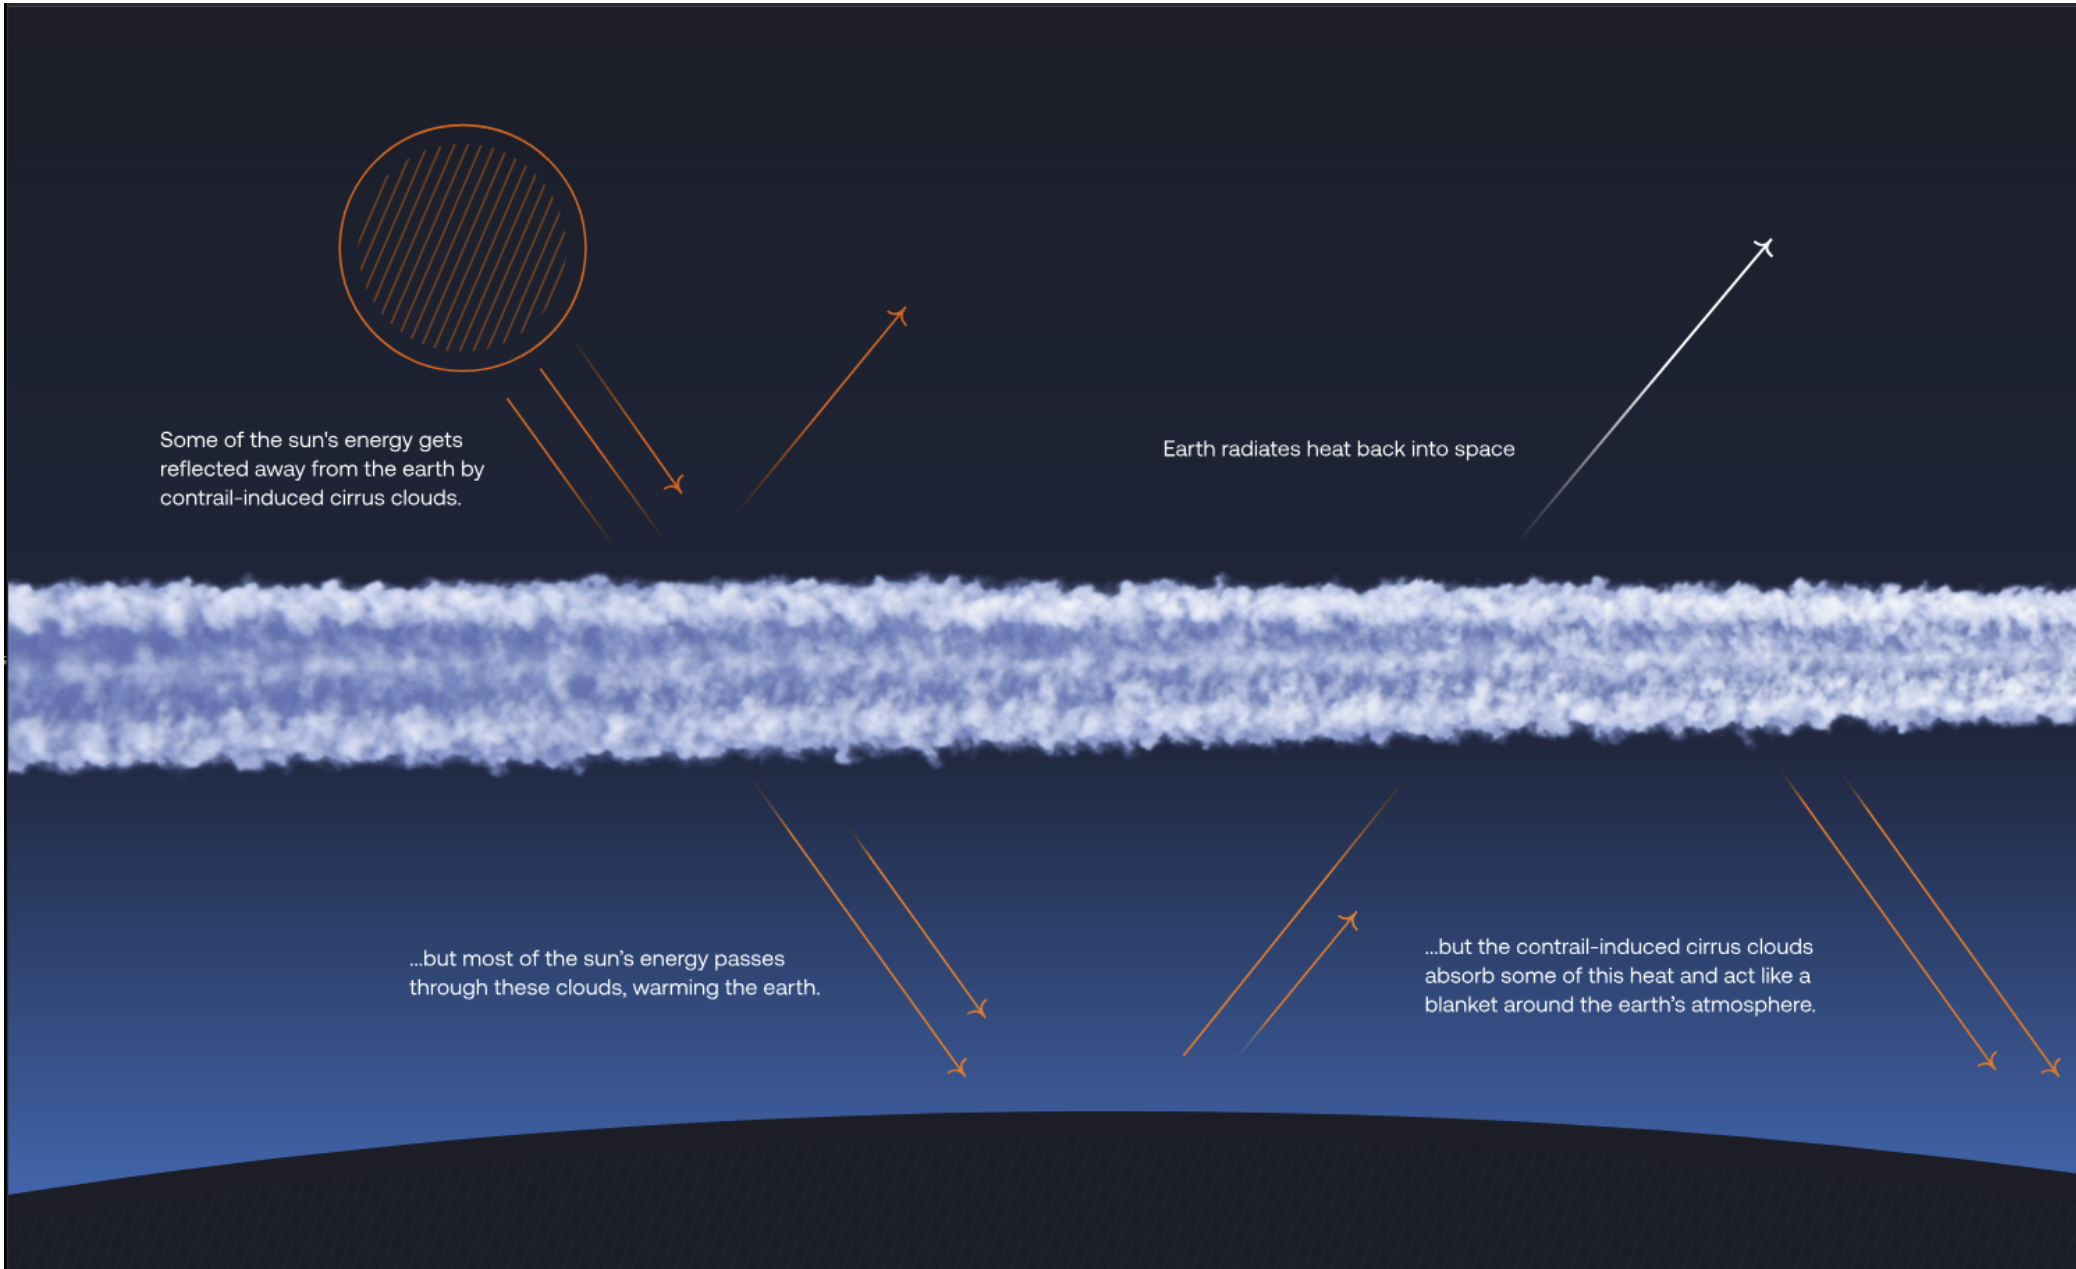
\includegraphics[width=0.9\linewidth]{figure1.png}  
    \caption{Conceptual illustration of contrail radiative forcing. A contrail forming
    in the cold upper troposphere overlies a warmer lower atmosphere and surface. Because
    longwave emission scales as $\sigma T^4$, emission to space from the contrail layer is
    substantially weaker than surface emission, leading to a net longwave warming effect.
    The schematic emphasizes the role of the vertical temperature profile rather than
    providing a quantitative radiative transfer calculation.}
    \label{fig:contrail_radiation}
\end{figure}

\subsection{Role of Vertical Temperature Structure}

The sign and magnitude of contrail radiative forcing depend critically on the vertical
temperature profile of the atmosphere. In an idealized two-layer framework consisting of
a surface at temperature $T_s$ and an overlying contrail layer at temperature $T_c$, the
clear-sky outgoing longwave radiation may be approximated as
\begin{equation}
    F_{\text{clear}} \approx \sigma T_s^4,
\end{equation}
whereas in the presence of an optically thick contrail, the effective emission to space
is instead governed by
\begin{equation}
    F_{\text{contrail}} \approx \sigma T_c^4.
\end{equation}
Since $T_c \ll T_s$ in the upper troposphere, it follows that
\begin{equation}
    F_{\text{contrail}} < F_{\text{clear}},
\end{equation}
yielding a positive longwave radiative forcing. This simple derivation highlights that
contrail impacts are fundamentally tied to atmospheric thermal structure rather than
cloud coverage alone.

Although radiative transfer is not explicitly simulated in this study, the temperature
contrast embodied in Figure~\ref{fig:contrail_radiation} motivates a focus on
upper-tropospheric environments where contrails are both thermodynamically favored and
radiatively effective.

\subsection{Environmental Controls on Contrail Persistence}

Whether a contrail forms and persists depends sensitively on the surrounding atmospheric
environment. Persistent contrails are observed primarily in ice-supersaturated regions
where relative humidity with respect to ice (RHi) exceeds 100\%, allowing ice crystals to
grow rather than sublimate \cite{Schumann1996,Schumann2017Monograph,GierensSpichtinger2012}.
Static stability, commonly quantified by the Brunt--V\"ais\"al\"a frequency $N$, regulates vertical mixing
and plume dilution, while vertical wind shear controls lateral stretching and deformation of the exhaust plume
\cite{Schumann2017Monograph,Turner1973}.


These controls operate at spatial scales that are often unresolved in global atmospheric
models. As a result, plume-scale mixing and microphysical decay must be parameterized,
introducing uncertainty into estimates of contrail persistence and radiative forcing.

\subsection{Atmospheric Data and Contrail Modeling Framework}

To characterize the atmospheric environments associated with contrail formation, this
study uses ERA5 reanalysis data \cite{Hersbach2020} together with the \texttt{pycontrails}
modeling framework \cite{pycontrails}. 
ERA5 pressure-level temperature, humidity, and wind fields are used to compute relative
humidity over ice, Brunt--V\"ais\"al\"a frequency, and vertical wind shear in the upper troposphere
\cite{Hersbach2020,Holton2013}.
 These fields define the thermodynamic and dynamic background in which
contrail formation is expected to occur.

The \texttt{pycontrails} framework is used to generate gridded contrail diagnostics and
to collocate atmospheric conditions with contrail-relevant regions and times. Rather
than relying on satellite-based detection, this approach enables systematic and
physically consistent exploration of contrail environments across space and time using
reanalysis-driven inputs.

\subsection{Hierarchical Modeling Approach}

To bridge the gap between large-scale atmospheric conditions and unresolved plume-scale
processes, this work adopts a hierarchical computational approach. First, a reduced-order
one-dimensional plume model implemented in MATLAB represents the cross-plume evolution
of ice mass using diffusion and bulk microphysical tendencies. This model enables
systematic parameter sweeps in RHi, $N$, and shear $S$, the construction of phase diagrams,
and the derivation of empirical scaling laws for contrail lifetime.

Second, high-fidelity two-dimensional simulations performed in COMSOL provide spatially
resolved reference solutions. These simulations explicitly resolve plume advection,
shear-driven deformation, and diffusion, allowing direct comparison with reduced-order
diagnostics such as centerline decay and effective plume width.

ERA5-driven atmospheric conditions and \texttt{pycontrails}-based diagnostics anchor both
modeling components in realistic upper-tropospheric environments, linking plume-scale
behavior to meteorologically consistent contrail formation regimes.

\subsection{Objectives and Scope}

The objective of this study is to quantify how relative humidity over ice, static
stability, and vertical wind shear jointly control contrail plume persistence. By
combining ERA5 reanalysis, \texttt{pycontrails}-based atmospheric diagnostics, reduced-
order MATLAB modeling, and high-fidelity COMSOL simulations, the study seeks to identify
controlling regimes, derive physically interpretable scaling relationships, and clarify
the plume-scale processes most relevant for contrail persistence in the atmosphere.


\section{Reduced-Order Contrail Plume Model (MATLAB)}
\label{sec:matlab_model}

This section presents a reduced-order contrail plume model implemented in MATLAB to
isolate how three environmental controls, relative humidity with respect to ice
(RHi), static stability (Brunt--V\"ais\"al\"a frequency $N$), and vertical wind shear, 
$S$govern contrail persistence. The code is given at the end of the document.
\subsection{Modeling choices and scope}
\label{sec:matlab_scope}

Contrail evolution couples turbulence-driven mixing and dilution, thermodynamic control
through supersaturation, and ice microphysics. Fully resolving these processes in
three dimensions is expensive and typically requires advanced microphysics and turbulence
closures. For this simulation, a reduced model is appropriate because the primary objective
is to identify \emph{regimes} and \emph{sensitivity} to environmental parameters that can
later be compared against reanalysis-derived distributions and refined using higher-fidelity
simulation.

We therefore model a contrail cross-section through a one-dimensional scalar field
$q_i(y,t)$, interpreted as a bulk \emph{ice mixing ratio proxy} (\si{kg/kg}) as a function of
cross-plume coordinate $y$ and time $t$. Streamwise structure is not explicitly represented
at this level. Instead, the model focuses on the competition between:
\begin{itemize}
    \item \textbf{Cross-plume dilution/spreading} represented by an effective diffusion term.
    \item \textbf{Bulk microphysical growth/decay} represented by an RHi-dependent source term.
\end{itemize}
These two processes are sufficient to generate an interpretable persistence metric
$\tau_{\mathrm{persist}}$ and to construct phase diagrams in $(\mathrm{RHi},N,S)$.

\subsection{Governing equation}
\label{sec:matlab_pde}

The reduced model solves an advection-free diffusion--reaction equation for $q_i(y,t)$:
\begin{equation}
\frac{\partial q_i}{\partial t}
=
K(N,S)\,\frac{\partial^2 q_i}{\partial y^2}
+\mathcal{M}\!\left(q_i;\mathrm{RHi}\right),
\qquad y\in\left[-\frac{L_y}{2},\,\frac{L_y}{2}\right], \; t\ge 0.
\label{eq:pde}
\end{equation}

The diffusion term represents the net effect of turbulent mixing and shear-enhanced dispersion
as an \emph{effective} cross-plume diffusivity $K$.
The microphysical term $\mathcal{M}$ represents net sublimation when air is subsaturated with
respect to ice and net growth (weakly) when supersaturated. This structure is intentionally
minimal: it preserves the correct qualitative threshold behavior at RHi $\approx 100\%$ while
remaining simple enough for regime mapping and parametric fitting. The diffusion form and Gaussian spreading behavior follow classical results for scalar diffusion
and plume width growth \cite{Taylor1921,Fischer1979}, while shear-enhanced dispersion motivates treating
shear as an effective mixing amplifier in reduced closures \cite{Taylor1953}.


\subsection{Effective diffusivity closure $K(N,S)$}
\label{sec:matlab_K}

The model parameterizes mixing strength via an effective diffusivity that depends on stability
$N$ and shear $S$:
\begin{equation}
K(N,S)=K_0\left(1+k_S\frac{|S|}{S_{\mathrm{ref}}}\right)\left(1+k_N\frac{N_{\mathrm{ref}}}{\max(N,N_{\min})}\right).
\label{eq:K}
\end{equation}

This choice is based on two modeling decisions:

\begin{itemize}
\item \textbf{Shear sensitivity:} A larger velocity gradient increases deformation and
interfacial area, enhancing entrainment and effective lateral spreading. The factor
$\left(1+k_S|S|/S_{\mathrm{ref}}\right)$ introduces a monotone increase of $K$ with $|S|$.

\item \textbf{Stability sensitivity:} Static stability modulates vertical motions and mixing pathways.
Rather than resolving stratified turbulence explicitly, $N$ is treated as an environmental control knob that shifts effective mixing rates over realistic ranges
\cite{Turner1973,Holton2013}.
 The inverse dependence
$N_{\mathrm{ref}}/N$ is deliberately simple, algebraically convenient for sweeps, and subject to
later validation/calibration against COMSOL (where shear-driven deformation and transport are
resolved spatially).
\end{itemize}

The parameters used in the model are
\[
K_0 = 1.0~\si{m^2/s},\quad
N_{\mathrm{ref}} = 0.01~\si{s^{-1}},\quad
S_{\mathrm{ref}} = 0.01~\si{s^{-1}},\quad
k_N = 2.0,\quad
k_S = 2.0,\quad
N_{\min}=10^{-4}~\si{s^{-1}}.
\]
These values were selected to yield cross-plume widening on the order of tens of meters over
tens of minutes, consistent with early-stage plume dispersion magnitudes, while keeping the
sensitivity coefficients order-one so that $N$ and $S$ materially affect outcomes within the
sweep ranges.

\subsection{Bulk microphysics closure $\mathcal{M}(q_i;\mathrm{RHi})$}
\label{sec:matlab_micro}

A reduced microphysics tendency is applied as a piecewise linear function of RHi:
\begin{equation}
\mathcal{M}(q_i;\mathrm{RHi})=
\begin{cases}
-\lambda_{\mathrm{decay}}(\mathrm{RHi})\,q_i, & \mathrm{RHi}<100\%,\\[4pt]
+\lambda_{\mathrm{grow}}(\mathrm{RHi})\,q_i, & \mathrm{RHi}>100\%,\\[4pt]
0, & \mathrm{RHi}=100\%,
\end{cases}
\label{eq:micro_piecewise}
\end{equation}
with
\begin{equation}
\lambda_{\mathrm{decay}}(\mathrm{RHi})=\dfrac{1-\mathrm{RHi}/100}{\tau_{\mathrm{micro}}},
\qquad
\lambda_{\mathrm{grow}}(\mathrm{RHi})=\gamma\,\dfrac{\mathrm{RHi}/100-1}{\tau_{\mathrm{micro}}}.
\label{eq:micro_rates}
\end{equation}
Here $\tau_{\mathrm{micro}}$ is a microphysical e-folding timescale and $\gamma\ll 1$ reduces
growth strength relative to decay strength in this bulk proxy model. In the implementation,
$\tau_{\mathrm{micro}}=90~\si{s}$ and $\gamma=0.05$.

The objective is to represent the correct \emph{direction} of microphysical tendency with minimal
complexity:
\begin{itemize}
\item For $\mathrm{RHi}<100\%$, ice sublimates and $q_i$ decays exponentially.
\item For $\mathrm{RHi}>100\%$, supersaturation supports persistence; weak growth prevents the model from
forcing immediate decay when dilution is modest.
\end{itemize}
This closure is designed for regime identification and parameter sensitivity rather than detailed
particle-size evolution.

\subsection{Domain, initial condition, and boundary conditions}
\label{sec:matlab_bc}

The cross-plume domain has width $L_y=200~\si{m}$ and is discretized with $N_y=201$ points,
so $\Delta y=L_y/(N_y-1)$. The initial plume is Gaussian:
\begin{equation}
q_i(y,0)=q_{i,0}\exp\!\left(-\frac{y^2}{2\sigma_y^2}\right),
\label{eq:ic}
\end{equation}
with $q_{i,0}=10^{-5}~\si{kg/kg}$ and $\sigma_y=15~\si{m}$.

At the domain boundaries, a no-flux condition is applied:
\begin{equation}
\frac{\partial q_i}{\partial y}\bigg|_{y=\pm L_y/2}=0,
\label{eq:bc}
\end{equation}
implemented numerically as a Neumann-type mirrored boundary (ghost-cell) approximation. The finite
domain and no-flux boundary prevent artificial mass loss at the edges, under the assumption that the
domain is sufficiently wide that the plume remains interior over the simulation window.

\subsection{Numerical implementation and stability}
\label{sec:matlab_numerics}

Equation \eqref{eq:pde} is solved using second-order centered finite differences for $\partial^2/\partial y^2$
and forward Euler time integration. For explicit diffusion, the timestep is constrained by the standard
stability criterion\cite{Fischer1979}:
\begin{equation}
\Delta t \le C_{\mathrm{FL}}\frac{\Delta y^2}{K(N,S)},
\label{eq:cfl}
\end{equation}
with a safety factor $C_{\mathrm{FL}}=0.45$. For each run, $\Delta t$ is computed from \eqref{eq:cfl}, the number
of steps is set so that the integration ends exactly at $t_{\mathrm{end}}=1800~\si{s}$, and non-negativity is enforced
by clamping $q_i\ge 0$ after each update. This approach ensures stable and consistent integration across large sweeps
without manual timestep tuning.

\subsection{Diagnostics and persistence definition}
\label{sec:matlab_diagnostics}

Three diagnostic outputs are used throughout the analysis:

\paragraph{Centerline persistence lifetime.}
Contrail lifetime is defined as the first time the centerline value drops below a fraction $\alpha$ of its initial
value:
\begin{equation}
\tau_{\mathrm{persist}}=\min\left\{t:\;q_i(0,t) < \alpha\,q_i(0,0)\right\},
\label{eq:tau_def}
\end{equation}
with $\alpha=0.20$. If the criterion is not met before $t_{\mathrm{end}}$, then $\tau_{\mathrm{persist}}$ is capped at
$t_{\mathrm{end}}=1800~\si{s}$.

\paragraph{Total ice proxy.}
A domain-integrated proxy for ice content is computed as
\begin{equation}
Q_i(t)=\int_{-L_y/2}^{L_y/2} q_i(y,t)\,dy.
\label{eq:Qi}
\end{equation}
This distinguishes microphysical changes (which modify $Q_i$) from pure redistribution by diffusion (which preserves
$Q_i$ in the absence of $\mathcal{M}$).

\paragraph{Effective plume width.}
A second-moment width is computed as
\begin{equation}
w(t)=\left[\frac{\int (y-\bar{y})^2 q_i(y,t)\,dy}{\int q_i(y,t)\,dy}\right]^{1/2},
\qquad
\bar{y}(t)=\frac{\int y\,q_i(y,t)\,dy}{\int q_i(y,t)\,dy}.
\label{eq:width}
\end{equation}
This provides a robust measure of spreading and connects to diffusion expectations (e.g.\ $w^2 \sim w_0^2 + 2Kt$) \cite{Taylor1921,Fischer1979}
when microphysical tendencies are weak.

\subsection{Sweep design and regime classification}
\label{sec:matlab_sweeps}

The MATLAB study uses three complementary sweep types:
\begin{enumerate}
    \item \textbf{Coarse sweep table} over $(\mathrm{RHi},N,S)\in\{90,100,110\}\times\{0.005,0.010\}\times\{0.002,0.010\}$
    to establish baseline sensitivities.
    \item \textbf{One-dimensional sweeps} varying one control while holding the other two fixed. For $N$ and $S$ sweeps,
    RHi is set to $95\%$ to ensure microphysical decay is active and dynamical dilution can modulate lifetime.
    \item \textbf{Two-dimensional regime mapping} in $(\mathrm{RHi},N)$ at fixed $S=0.005~\si{s^{-1}}$ to identify persistence
    boundaries.
\end{enumerate}

A persistence threshold of $\tau_{\mathrm{persist}}\ge 600~\si{s}$ (10 minutes) is used to classify cases as
\emph{persistent} vs.\ \emph{short-lived} for phase-diagram interpretation. This binary regime definition is convenient
for later comparison against ERA5/\texttt{pycontrails}-derived persistence indicators.

\subsection{MATLAB results figures}
\label{sec:matlab_figs}

Figures~\ref{fig:matlab_sweeps}--\ref{fig:matlab_mech_fit} summarize the reduced-model behavior. All figures are direct
outputs from \texttt{contrail\_plume\_model.m}.

% ============================================================
% Composite Figure A — 1D sweeps (1.jpg, 2.jpg, 3.jpg)
% ============================================================
\begin{figure}[t]
    \centering
    \begin{subfigure}[b]{0.32\linewidth}
        \centering
        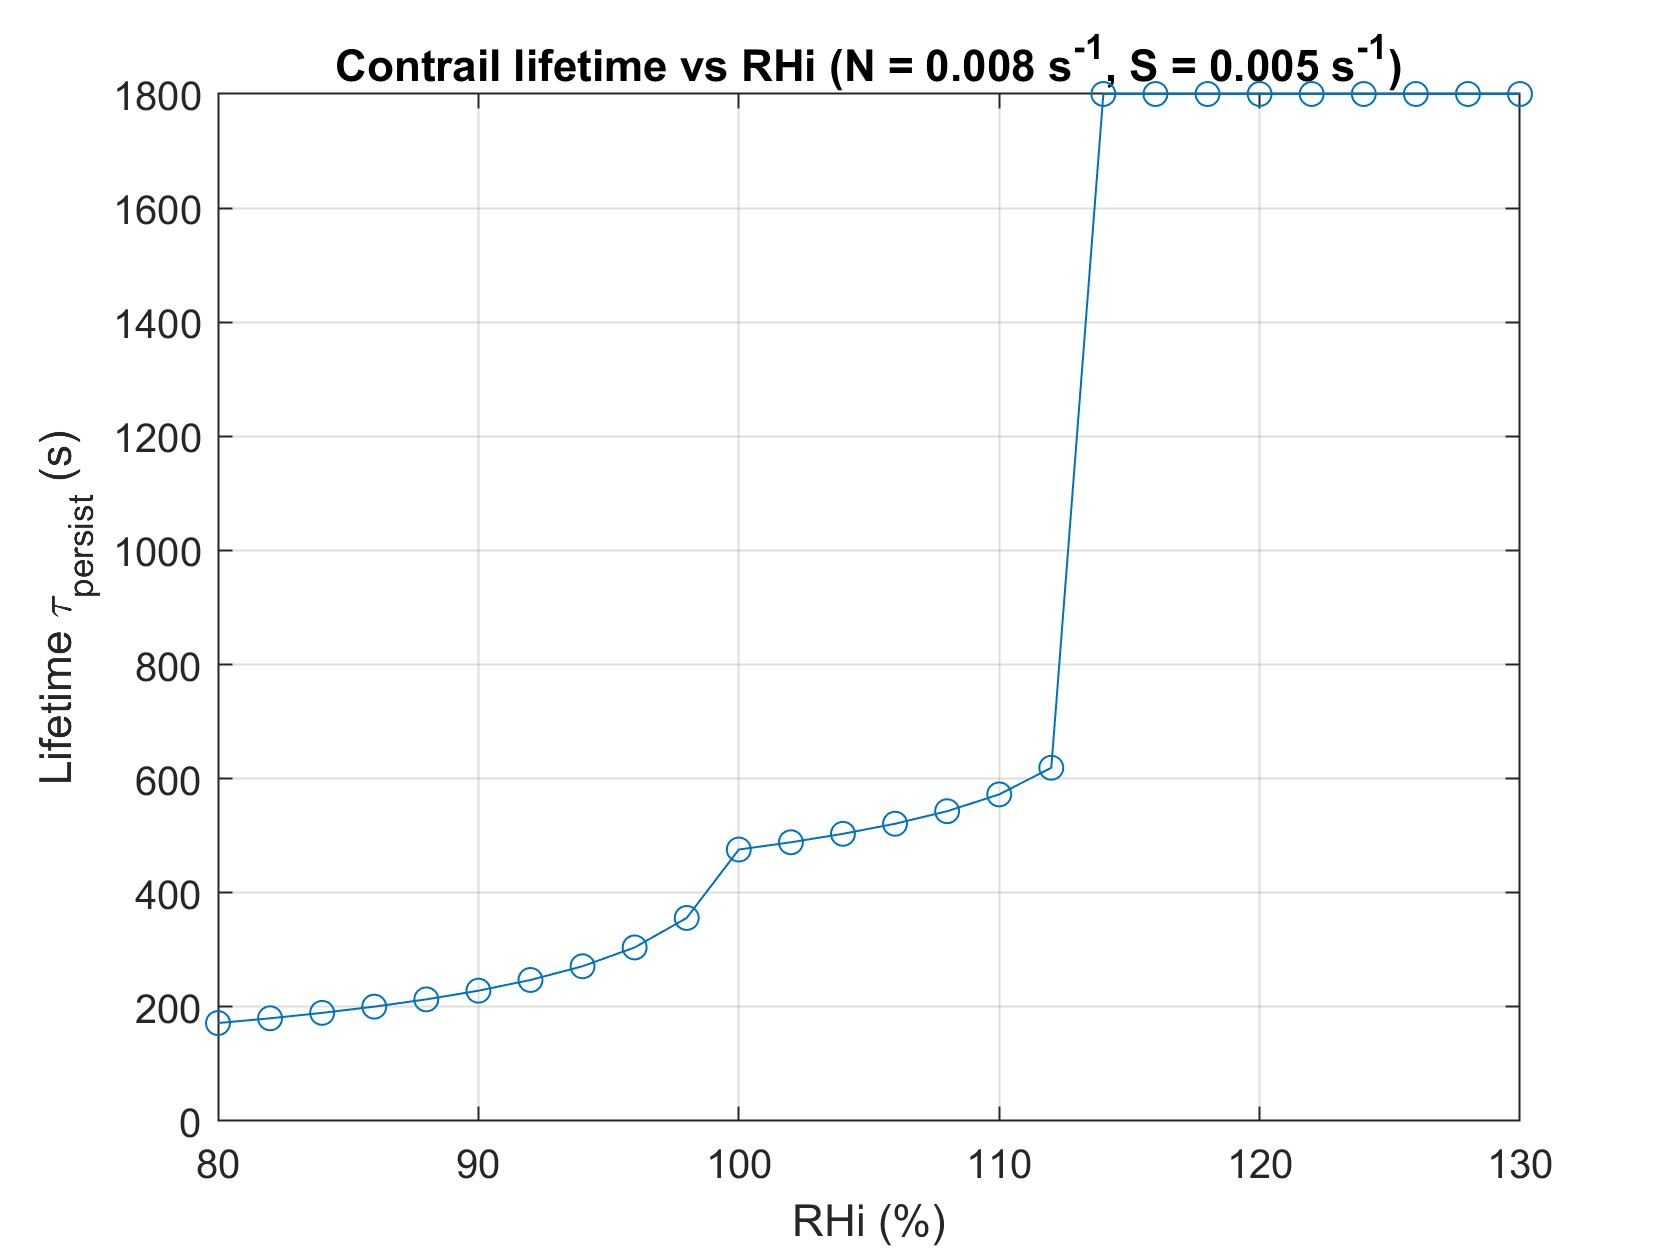
\includegraphics[width=\linewidth]{1.jpg}
        \caption{Lifetime vs RHi}
        \label{fig:sweep_RHi}
    \end{subfigure}
    \hfill
    \begin{subfigure}[b]{0.32\linewidth}
        \centering
        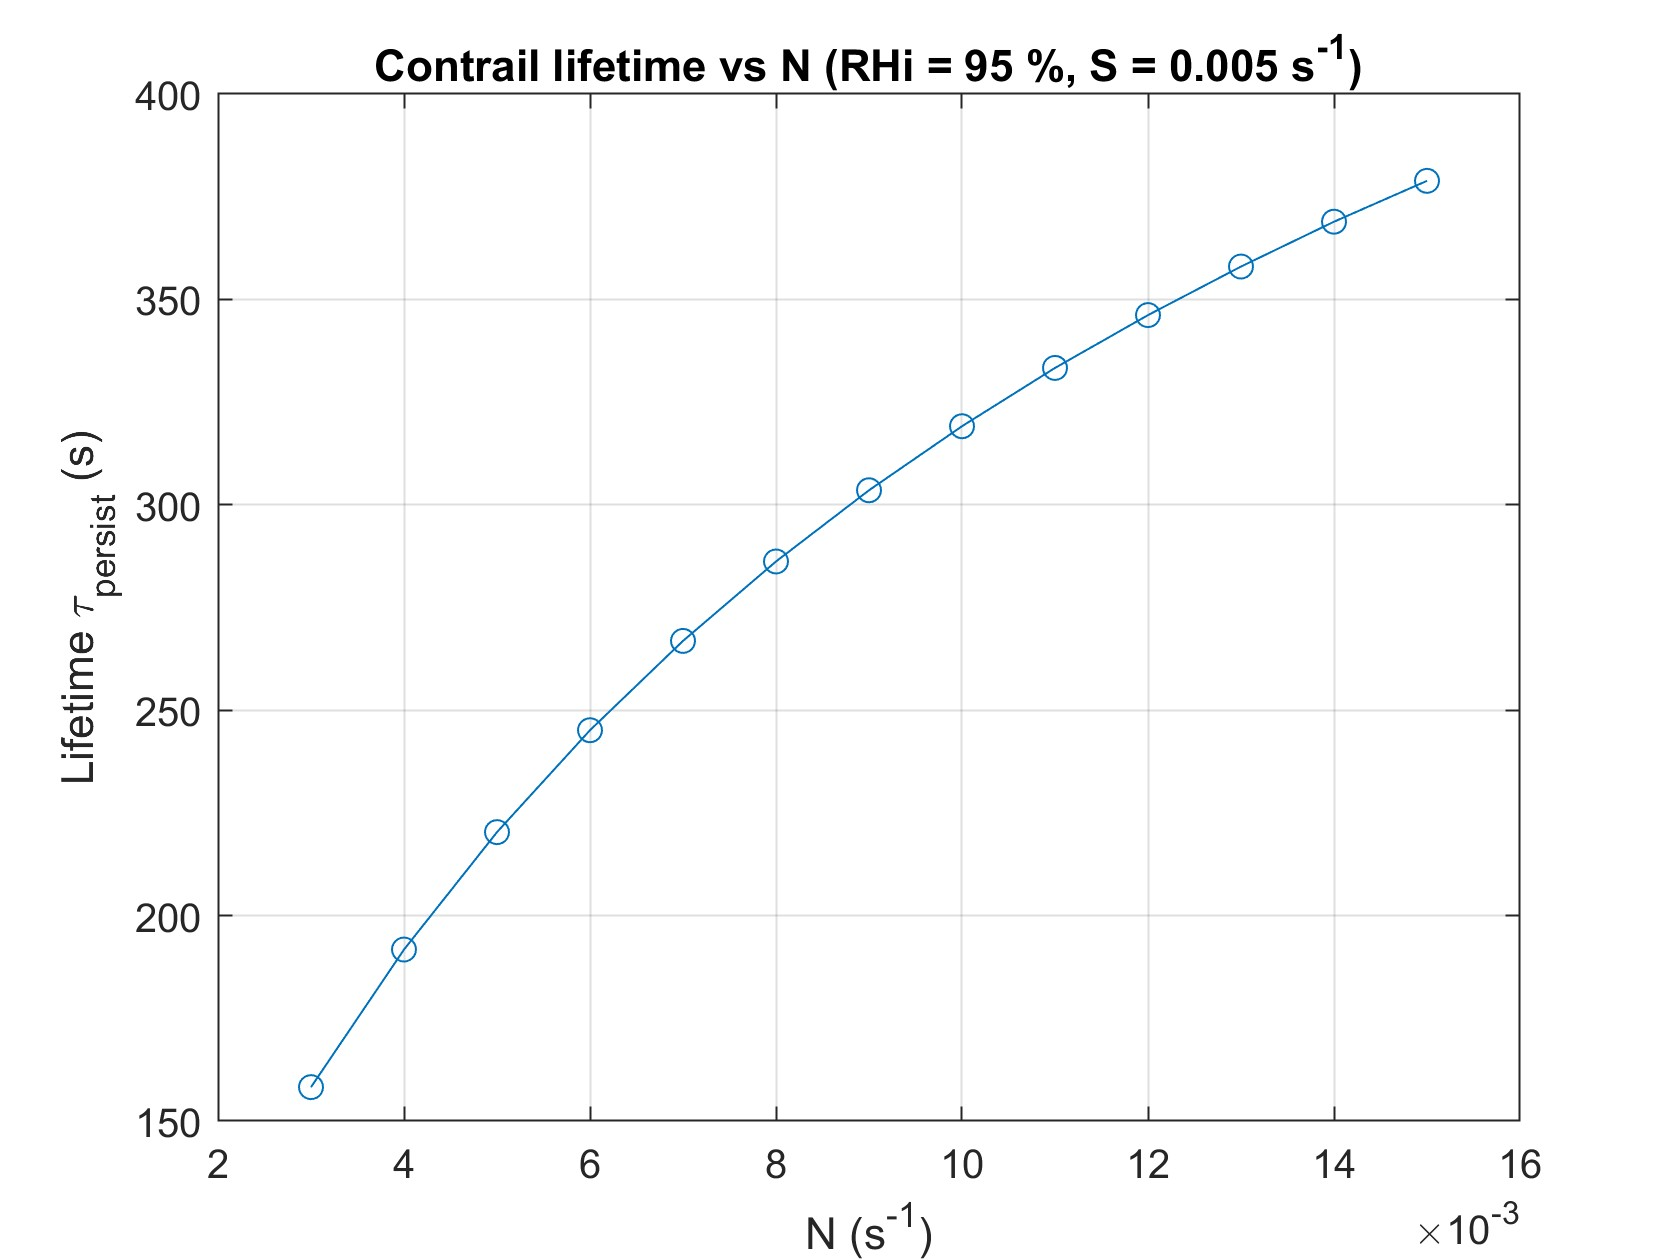
\includegraphics[width=\linewidth]{2.jpg}
        \caption{Lifetime vs $N$}
        \label{fig:sweep_N}
    \end{subfigure}
    \hfill
    \begin{subfigure}[b]{0.32\linewidth}
        \centering
        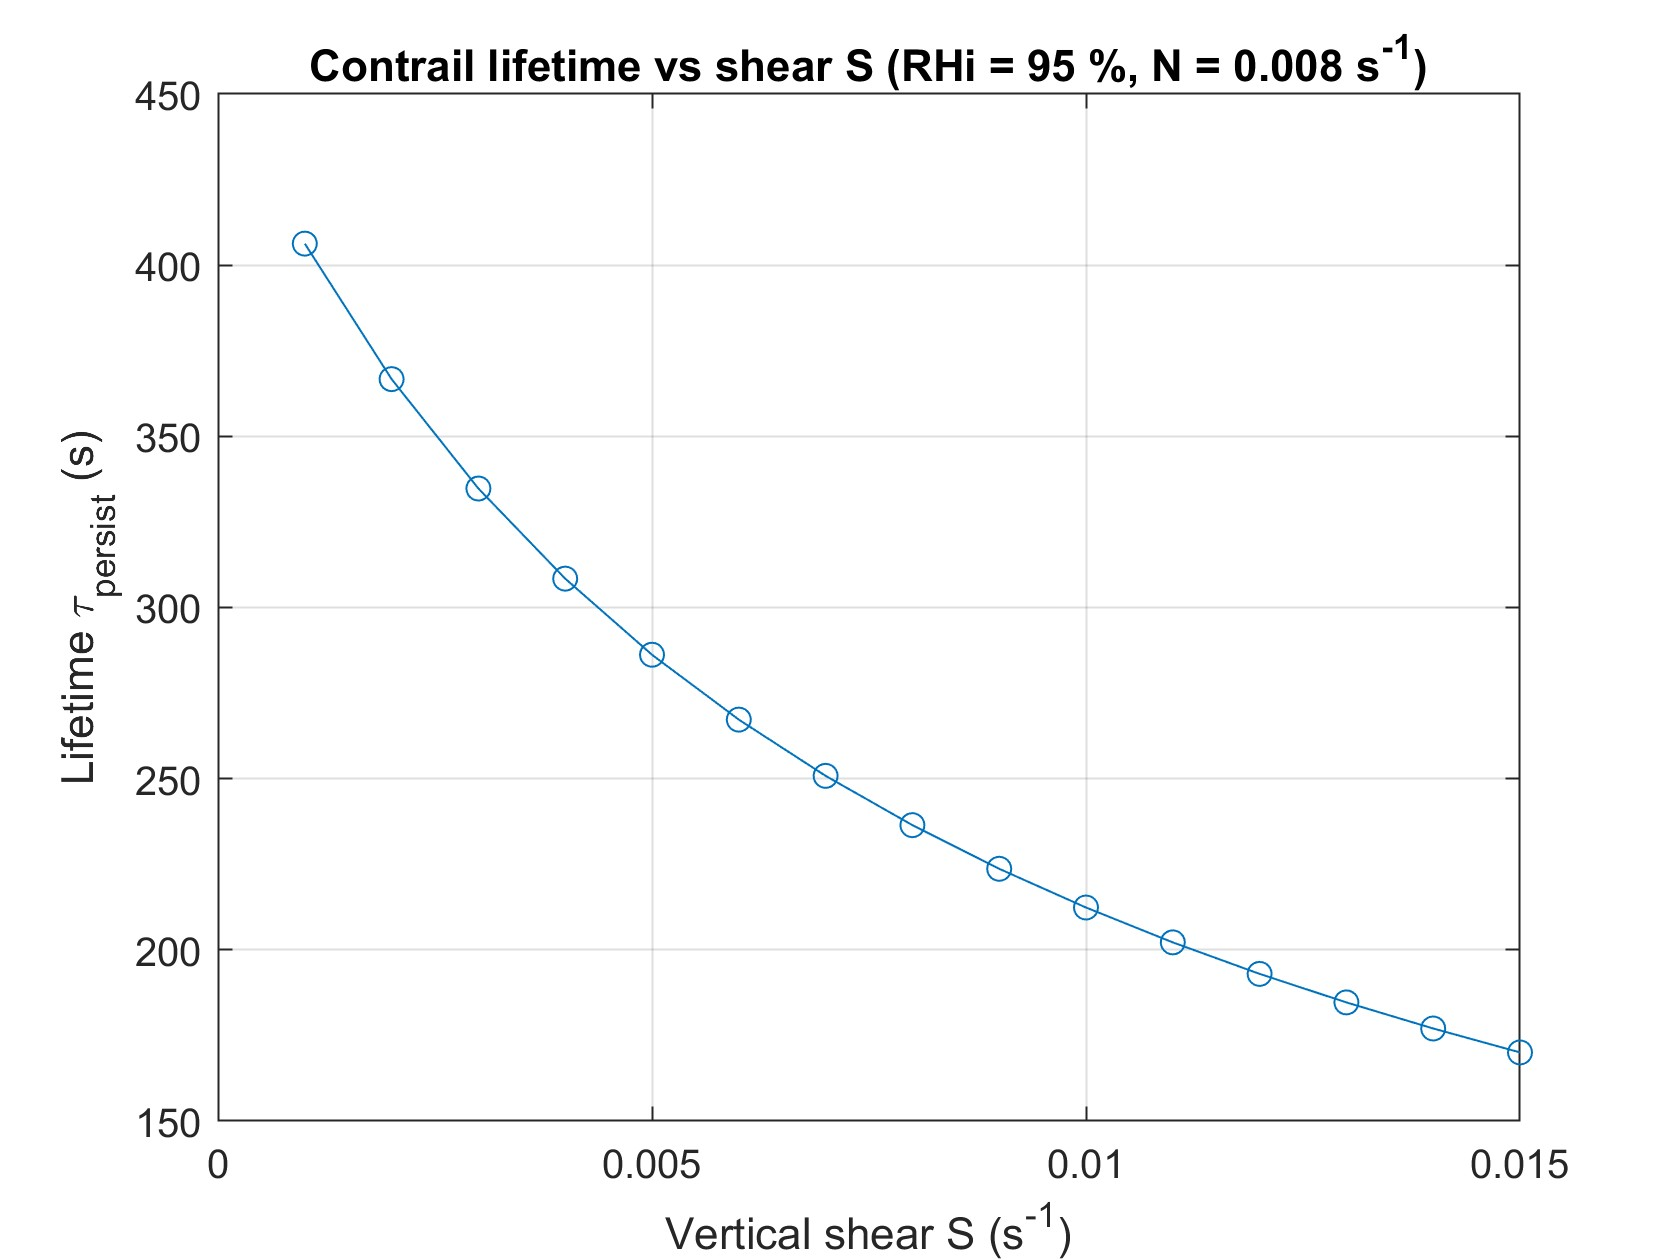
\includegraphics[width=\linewidth]{3.jpg}
        \caption{Lifetime vs $S$}
        \label{fig:sweep_S}
    \end{subfigure}

    \caption{One-dimensional sensitivity sweeps of persistence lifetime $\tau_{\mathrm{persist}}$ in the MATLAB reduced model.
    Panel (a) shows a sharp increase of lifetime with ice supersaturation (RHi), including cases that reach the simulation cap
    at $t_{\mathrm{end}}=1800~\si{s}$ for sufficiently high RHi.
    Panels (b) and (c) use marginal humidity ($\mathrm{RHi}=95\%$) so that microphysical decay is active and dynamical controls
    ($N$ and $S$ via $K(N,S)$) measurably modulate lifetime.}
    \label{fig:matlab_sweeps}
\end{figure}

% ============================================================
% Composite Figure B — 2D phase diagram (4.jpg, 5.jpg)
% ============================================================
\begin{figure}[h!]
    \centering
    \begin{subfigure}[h!]{0.48\linewidth}
        \centering
        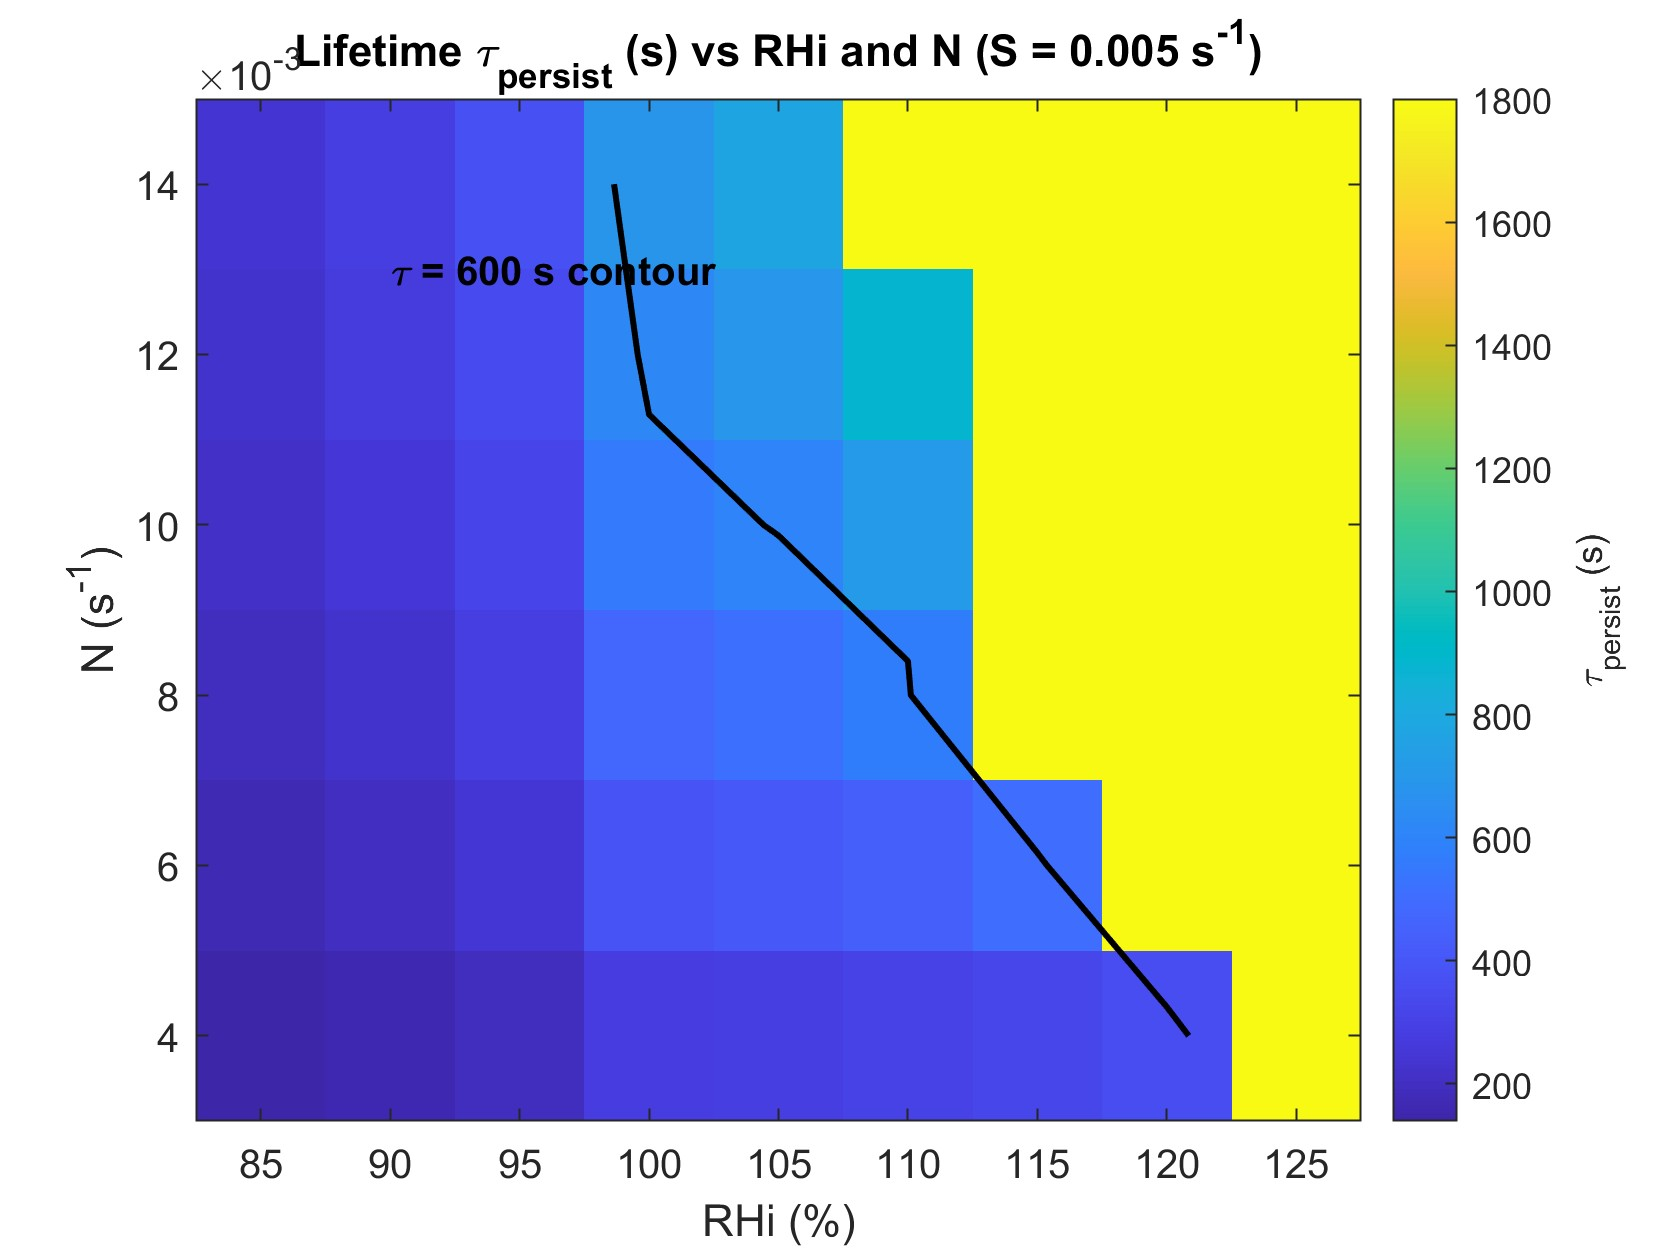
\includegraphics[width=\linewidth]{4.jpg}
        \caption{Lifetime map $\tau_{\mathrm{persist}}$}
        \label{fig:phase_tau}
    \end{subfigure}
    \hfill
    \begin{subfigure}[h!]{0.48\linewidth}
        \centering
        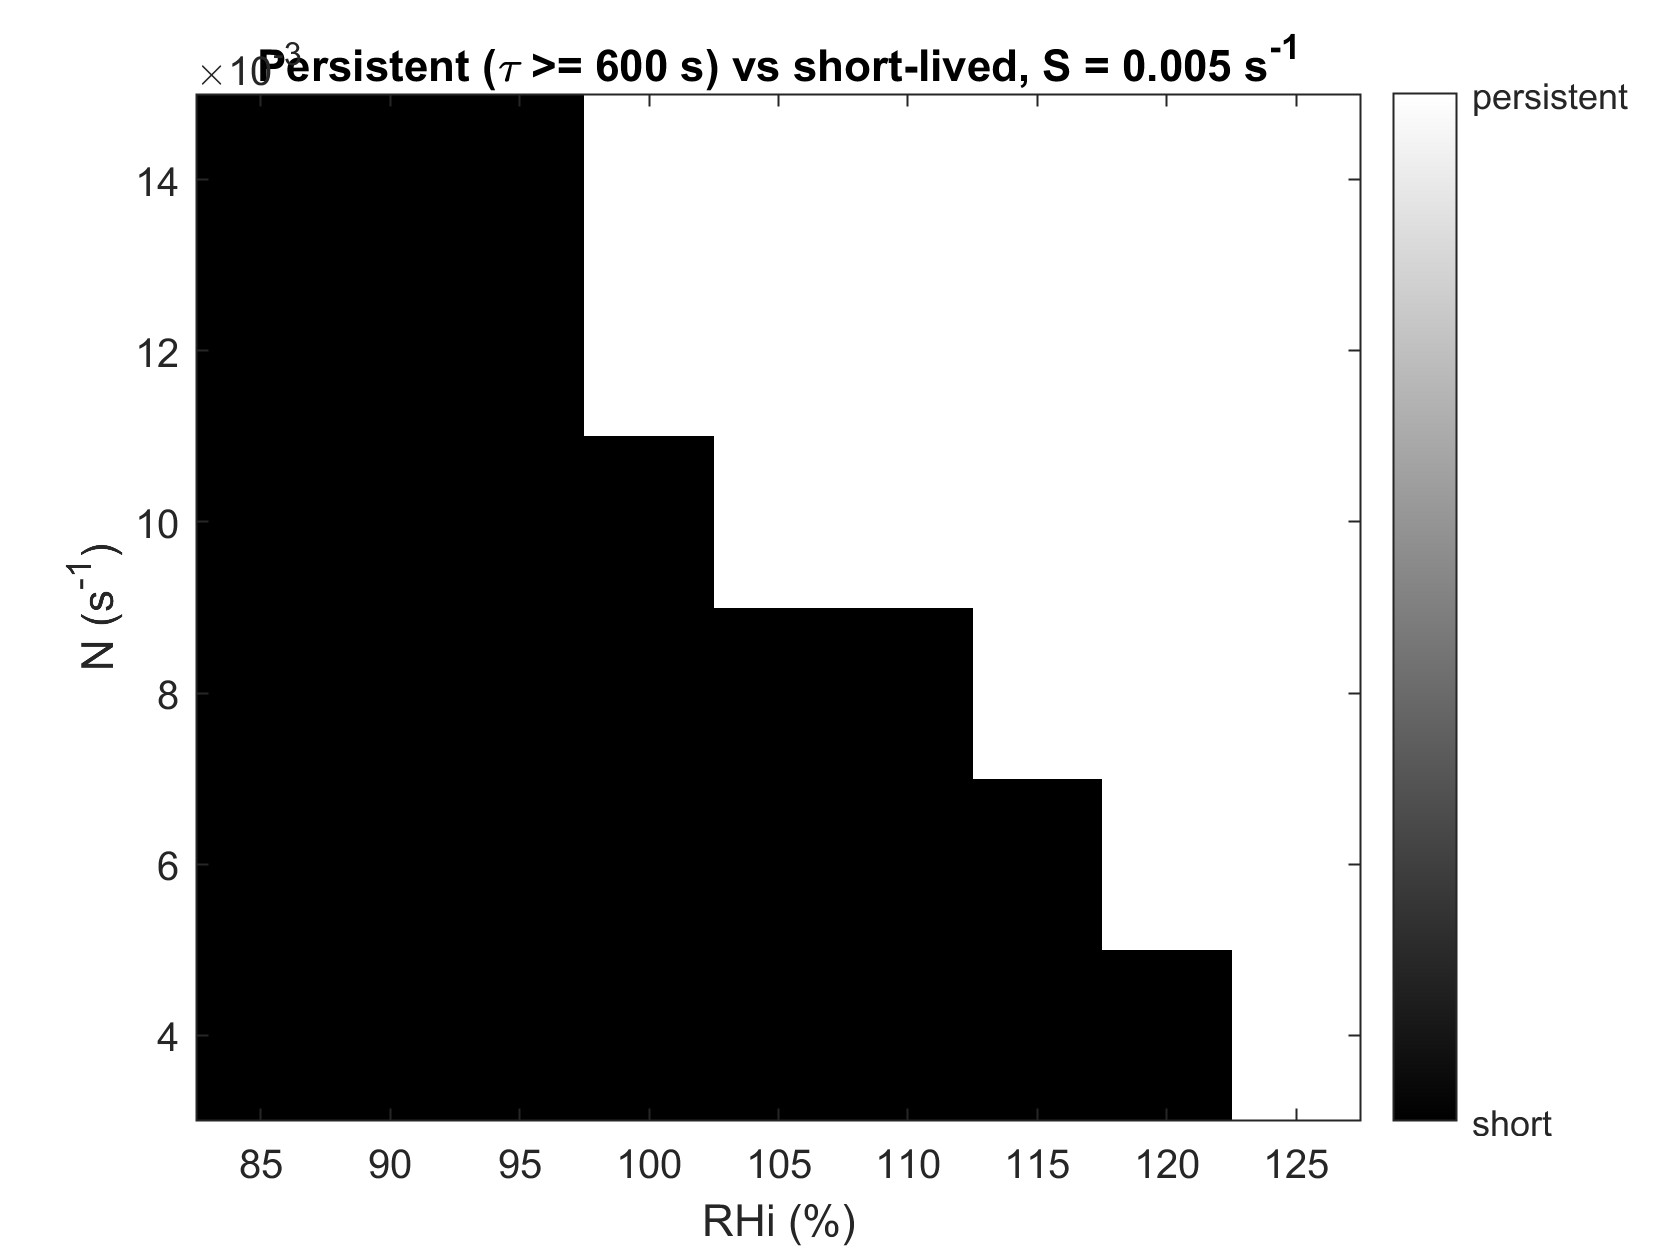
\includegraphics[width=\linewidth]{5.jpg}
        \caption{Persistent vs short-lived}
        \label{fig:phase_binary}
    \end{subfigure}

    \caption{Regime behavior in $(\mathrm{RHi},N)$ space at fixed $S=0.005~\si{s^{-1}}$.
    (a) Lifetime phase map with the $\tau_{\mathrm{persist}}=600~\si{s}$ contour overlaid.
    (b) Binary regime classification using the same $600~\si{s}$ persistence threshold.
    The resulting boundary highlights a nonlinear transition governed primarily by RHi and modulated by dynamical dilution
    through the $N$-dependence of $K(N,S)$.}
    \label{fig:matlab_phase}
\end{figure}

% ============================================================
% Composite Figure C — Mechanism + closure (6.jpg, 7.jpg, 8.jpg)
% ============================================================
\begin{figure}[h!]
    \centering
    \begin{subfigure}[h!]{0.48\linewidth}
        \centering
        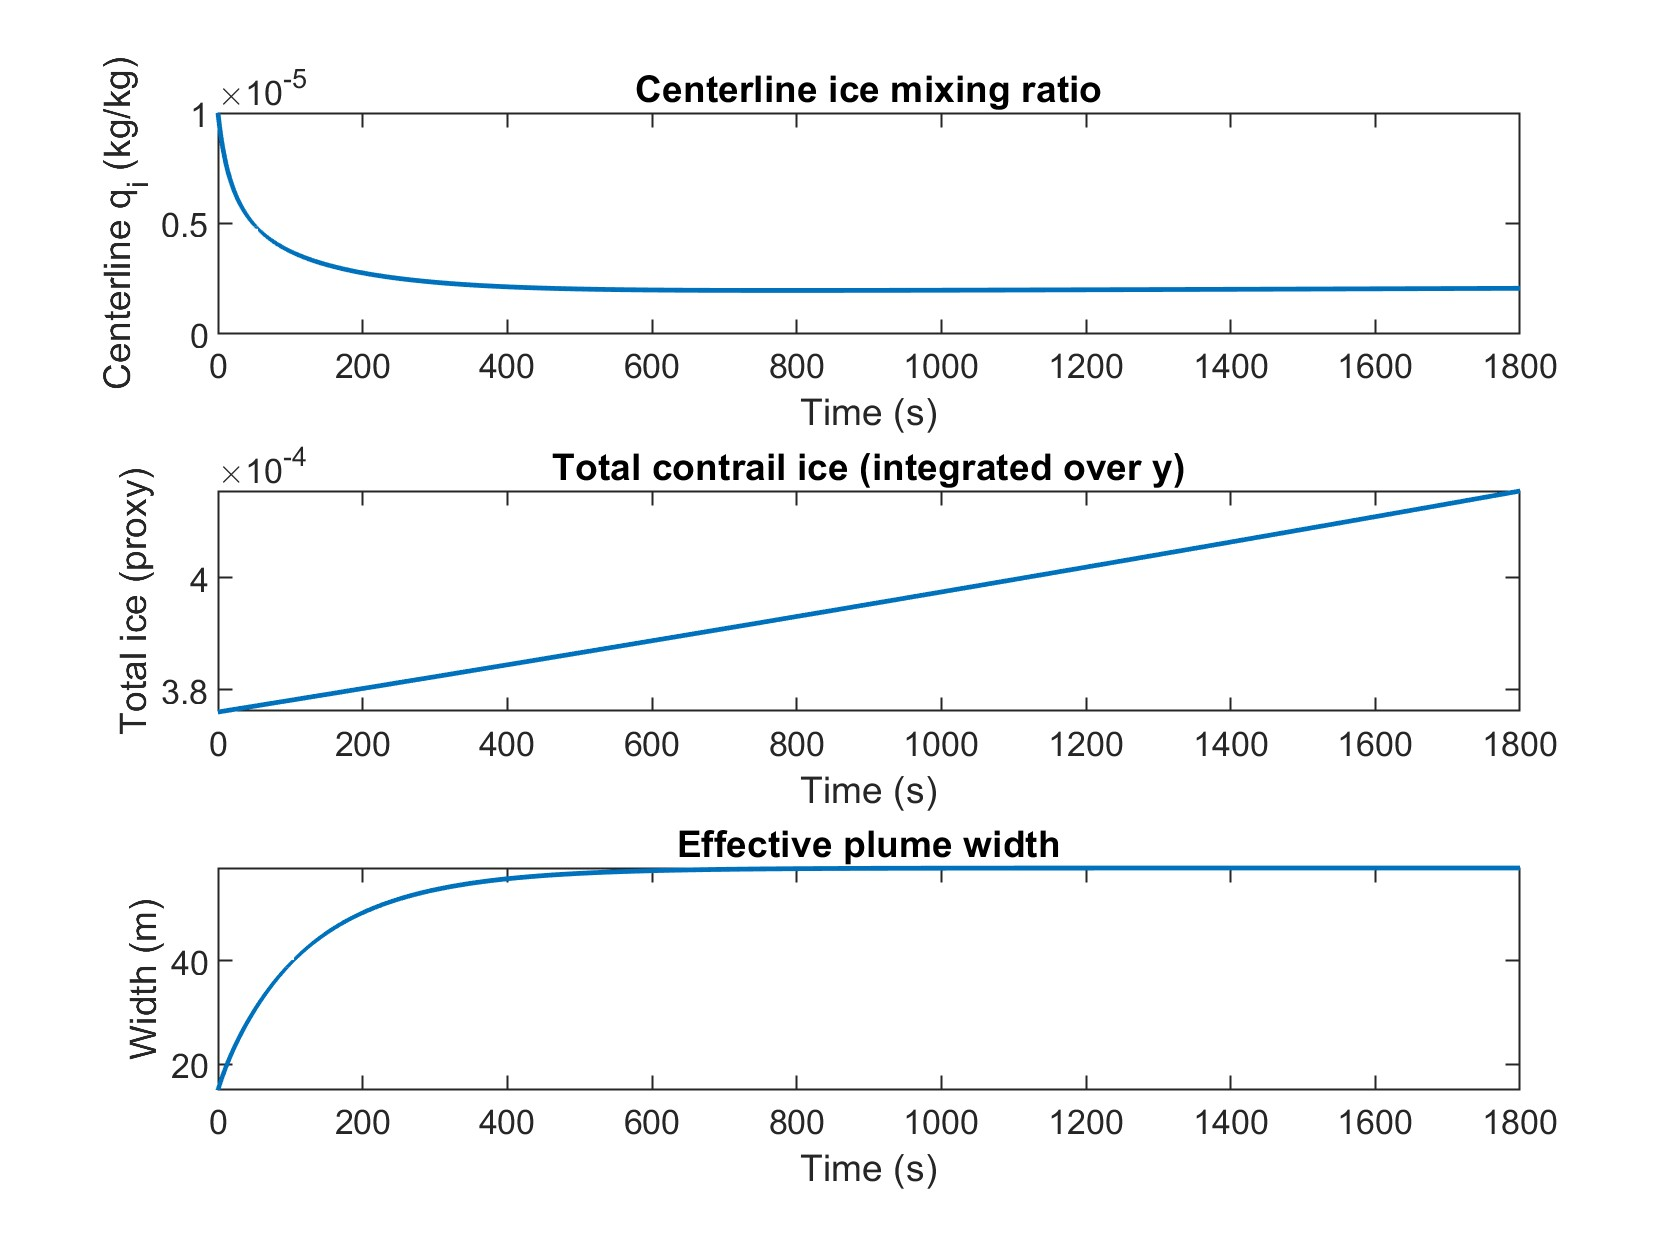
\includegraphics[width=\linewidth]{6.jpg}
        \caption{Time evolution diagnostics}
        \label{fig:demo_timeseries}
    \end{subfigure}
    \hfill
    \begin{subfigure}[h!]{0.48\linewidth}
        \centering
        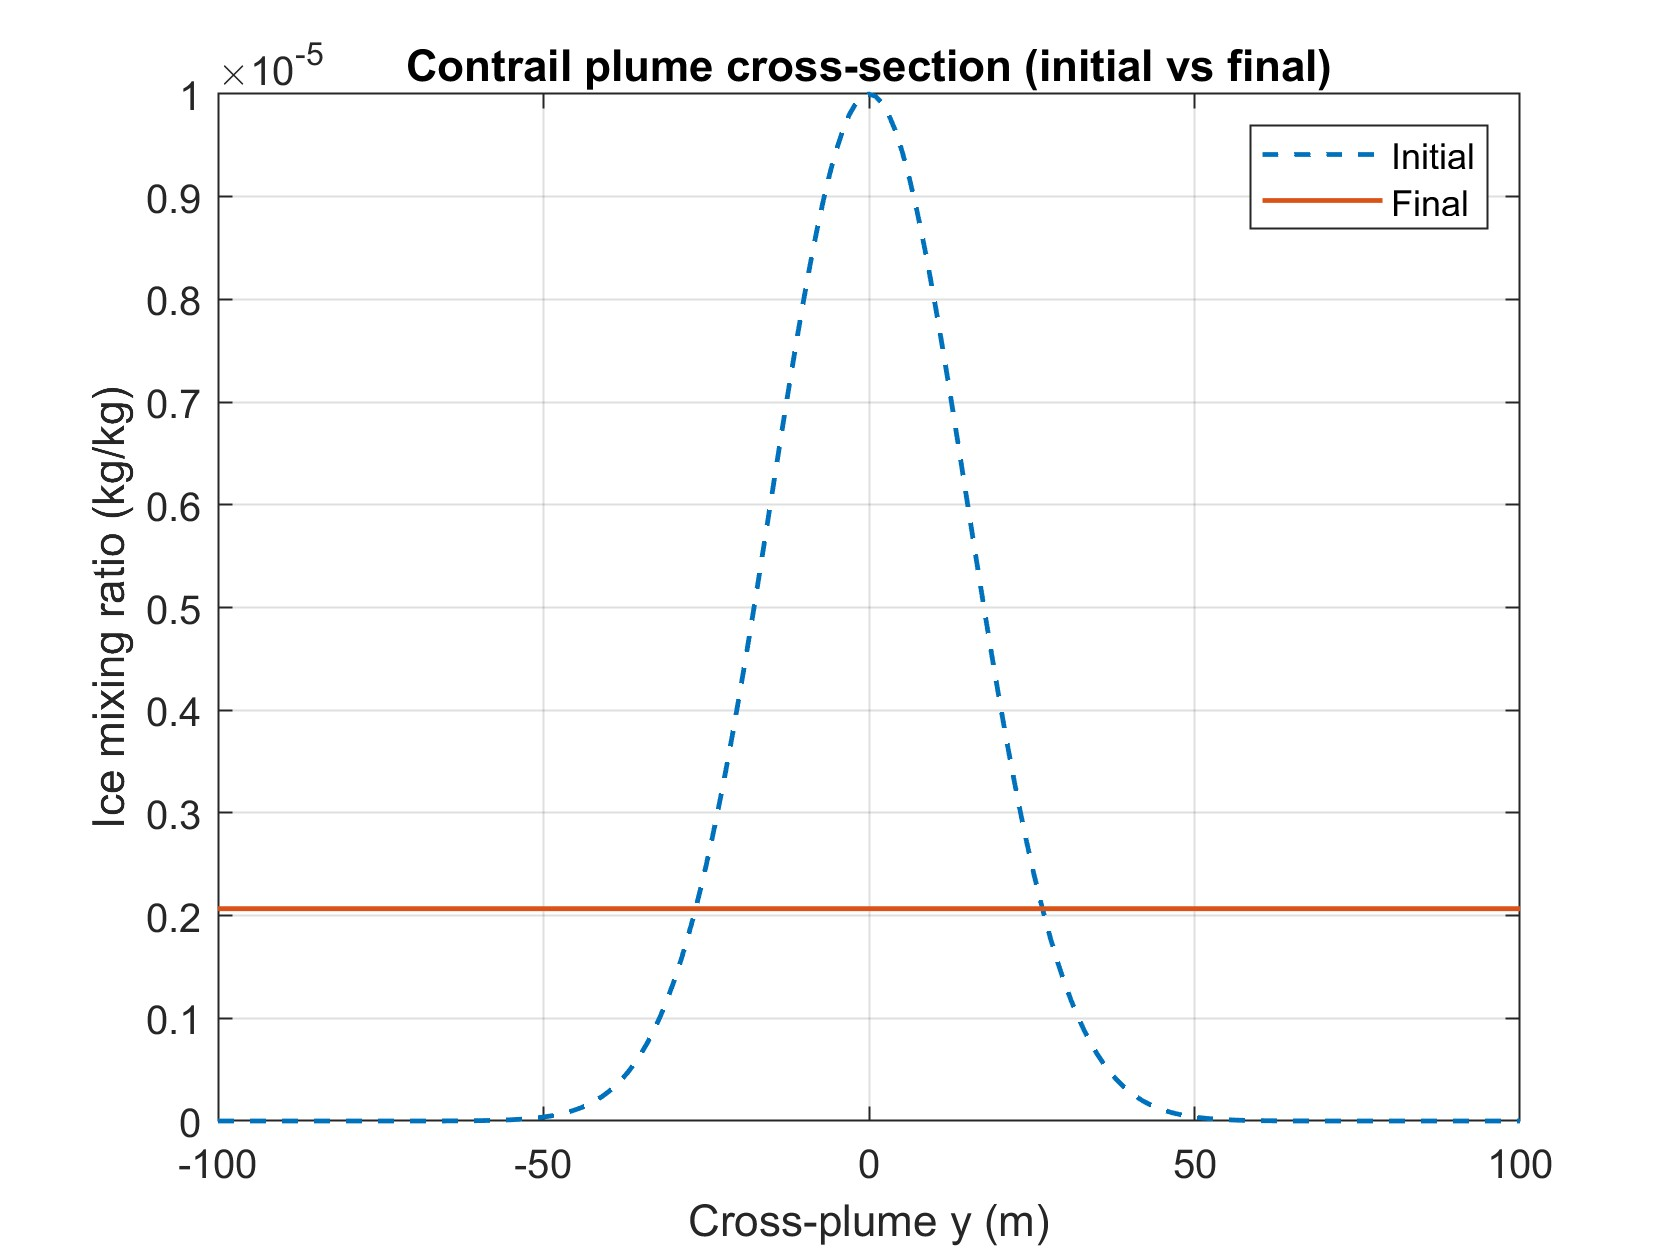
\includegraphics[width=\linewidth]{7.jpg}
        \caption{Initial vs final profile}
        \label{fig:demo_profile}
    \end{subfigure}

    \medskip

    \begin{subfigure}[h!]{0.65\linewidth}
        \centering
        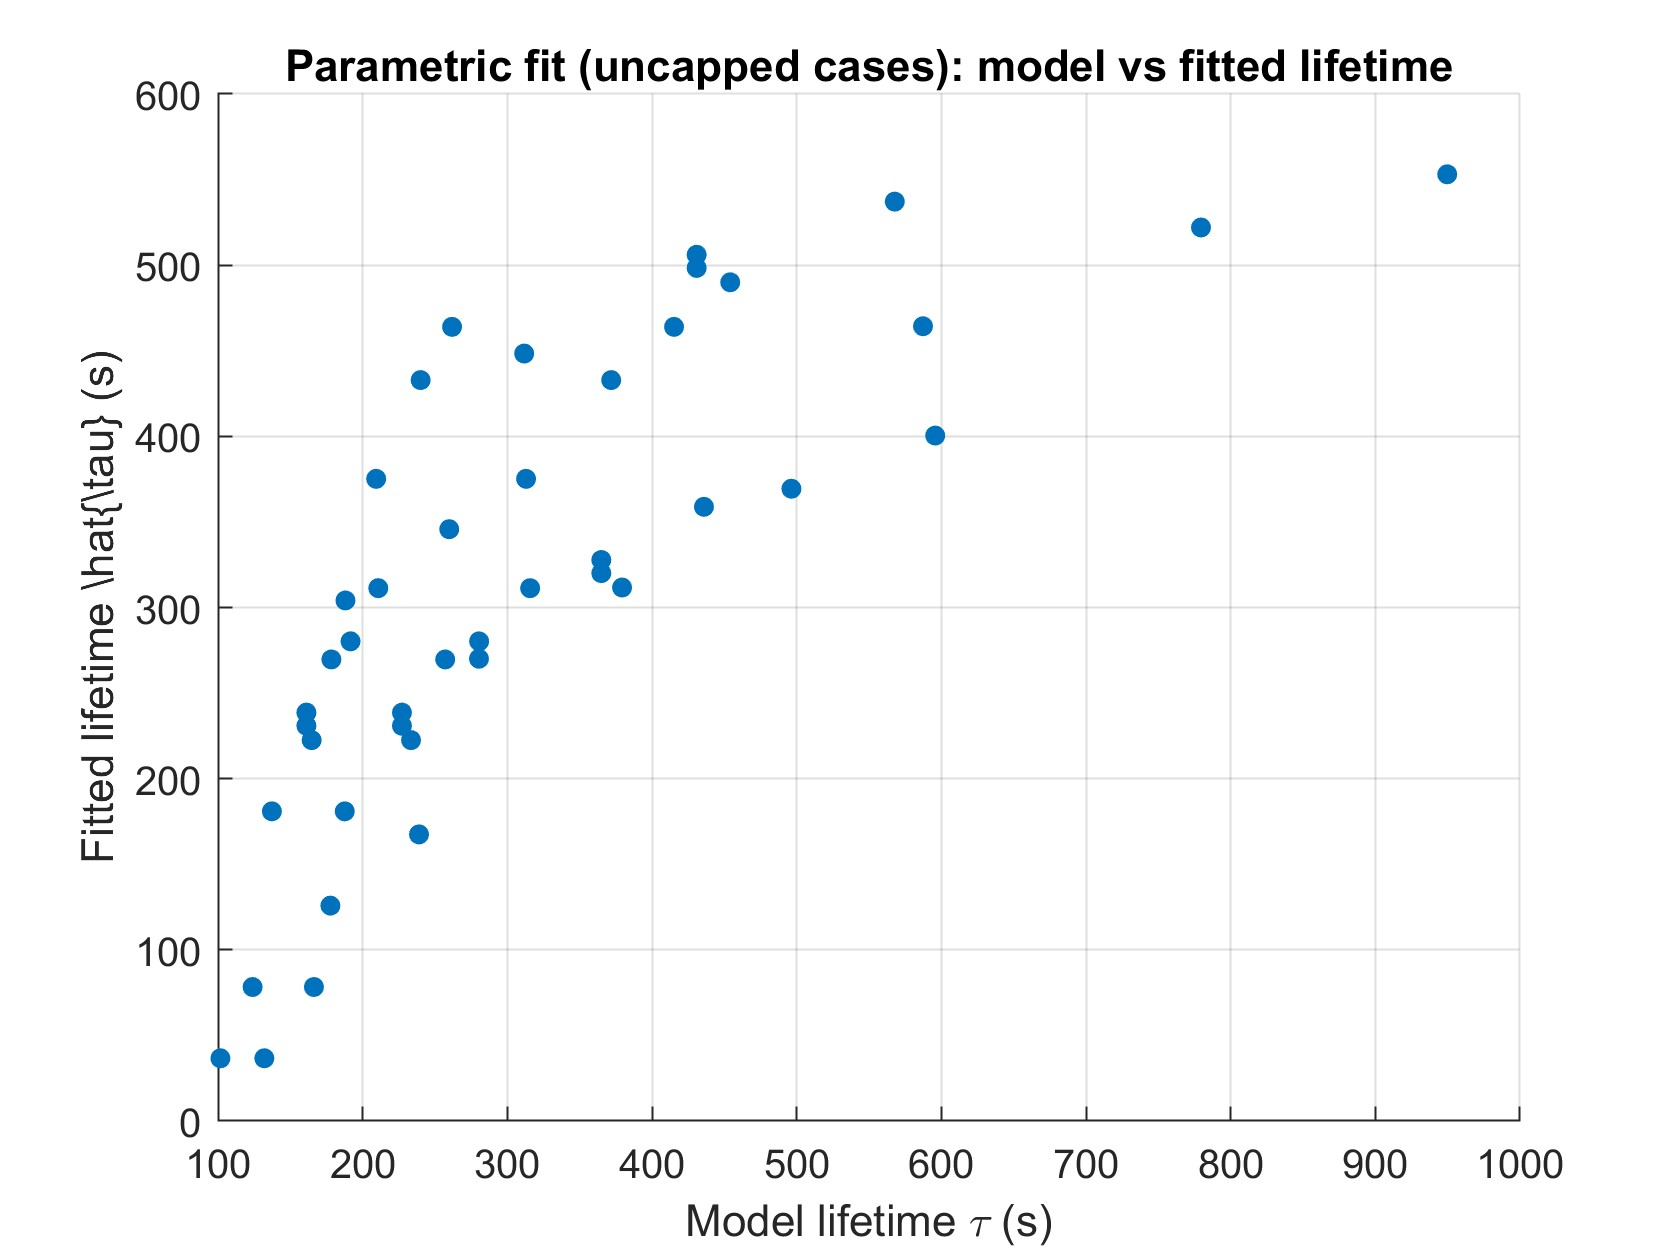
\includegraphics[width=\linewidth]{8.jpg}
        \caption{Parametric fit (uncapped cases)}
        \label{fig:param_fit}
    \end{subfigure}

    \caption{Mechanistic diagnostics and empirical closure for the MATLAB model.
    (a) Centerline $q_i(0,t)$, total ice proxy $Q_i(t)$, and plume width $w(t)$ for a representative case
    $(\mathrm{RHi},N,S)=(110\%,\,0.005~\si{s^{-1}},\,0.002~\si{s^{-1}})$.
    (b) Initial and final cross-plume profiles for the same case, illustrating dilution-driven reduction of the core amplitude,
    which underlies the persistence definition in \eqref{eq:tau_def}.
    (c) Comparison of modeled lifetimes to fitted lifetimes for uncapped cases, supporting a compact empirical lifetime law
    used as a summary statistic within the explored parameter range.}
    \label{fig:matlab_mech_fit}
\end{figure}

\subsection{Recorded MATLAB command-window output}
\label{sec:matlab_console}

The MATLAB command-window output from the coarse sweep,
the detailed demo case, and the regression fit is reproduced below:

\begin{verbatim}
=== Basic parameter sweep: lifetime vs (RHi, N, S) ===
RHi(%)  N (s^-1)  S (s^-1)  Lifetime (s)
   90    0.0050   0.0020      228.4
   90    0.0050   0.0100      136.2
   90    0.0100   0.0020      310.3
   90    0.0100   0.0100      194.1
  100    0.0050   0.0020      475.8
  100    0.0050   0.0100      222.0
  100    0.0100   0.0020      793.0
  100    0.0100   0.0100      370.1
  110    0.0050   0.0020      572.4
  110    0.0050   0.0100      237.4
  110    0.0100   0.0020     1800.0
  110    0.0100   0.0100      420.2

=== Detailed demo case ===
RHi = 110 %, N = 0.0050 s^-1, S = 0.0020 s^-1
Estimated contrail lifetime: 572.4 s

=== Regression fit for tau_persist(RHi, N, S) ===
Fitted coefficients (using 43 / 48 samples):
tau = a0 + a1*(RHi-100)_+ + a2*N^{-1} + a3*|S|^{-1}
a0 = 300.377 s
a1 = 17.831 s / percent
a2 = -1.346 s^2
a3 = 0.801 s^2
RMSE of fit (uncapped lifetimes only): 112.92 s
\end{verbatim}

\subsection{Empirical lifetime law (regression summary)}
\label{sec:matlab_regression}

To provide a compact summary statistic for the reduced-model behavior within the explored parameter
range, an empirical law was fit to simulated lifetimes using a simple linear regression on
hand-crafted features:
\begin{equation}
\hat{\tau}
=
a_0
+
a_1(\mathrm{RHi}-100)_+
+
a_2 N^{-1}
+
a_3 |S|^{-1},
\qquad (x)_+ \equiv \max(x,0).
\label{eq:tau_fit}
\end{equation}
The fit was performed on \emph{uncapped} cases only ($\tau_{\mathrm{persist}}<t_{\mathrm{end}}$) to avoid bias from
the artificial upper bound at $t_{\mathrm{end}}=1800~\si{s}$. The fitted coefficients and RMSE are listed in
Section~\ref{sec:matlab_console}. This regression is not asserted as a universal physical law; rather, it offers
an interpretable equation for rapid evaluation and for linking the reduced-model response surface to
ERA5/\texttt{pycontrails}-derived environmental distributions.

\section{High-Fidelity Plume Simulations (COMSOL)}
\label{sec:comsol}

The reduced-order MATLAB model presented in Section~\ref{sec:matlab_model} represents
plume spreading through a scalar effective diffusivity $K(N,S)$ and models persistence
via a centerline decay criterion. While this approach enables efficient regime mapping,
it does not explicitly resolve the spatial structure of the plume, shear-driven
deformation, or the coupled velocity--pressure dynamics of the flow. To evaluate the
validity of these assumptions and to provide a spatially resolved reference, we perform
high-fidelity numerical simulations using COMSOL Multiphysics.

The COMSOL simulations occupy an intermediate tier in a hierarchical modeling framework:
they are more physically resolved than the 1D reduced model, but still simplified
relative to full atmospheric large-eddy simulations. Their role is to resolve early-time
plume transport and dilution mechanisms and to provide diagnostics that can be directly
compared to those extracted from the MATLAB model.

\subsection{Governing equations}
\label{sec:comsol_equations}

The COMSOL simulations are performed on a two-dimensional Cartesian domain $(x,y)$.
The flow is modeled using the incompressible Navier--Stokes equations,
\begin{align}
\nabla \cdot \mathbf{u} &= 0, \label{eq:comsol_continuity} \\
\rho \left(
\frac{\partial \mathbf{u}}{\partial t}
+ \mathbf{u}\cdot\nabla \mathbf{u}
\right)
&= -\nabla p + \mu \nabla^2 \mathbf{u} + \mathbf{f},
\label{eq:comsol_momentum}
\end{align}
where $\mathbf{u}(x,y,t)$ is the velocity field, $p(x,y,t)$ is pressure, $\rho$ is air
density, and $\mu$ is the dynamic viscosity. A prescribed forcing $\mathbf{f}$ and/or
boundary conditions are used to establish a controlled inflow and vertical shear.

Transport of a plume-linked scalar $c(x,y,t)$ is governed by an advection--diffusion--decay
equation,
\begin{equation}
\frac{\partial c}{\partial t}
+ \mathbf{u}\cdot\nabla c
=
\nabla\cdot\left(D\nabla c\right)
- \lambda c,
\label{eq:comsol_scalar}
\end{equation}
where $D$ is a diffusivity and $\lambda$ is a bulk decay rate. The scalar $c$ serves as a
proxy for exhaust or ice-related quantities and is used to quantify plume dilution and
persistence. Equation~\eqref{eq:comsol_scalar} is the spatially resolved analogue of the
reduced-order evolution equation \eqref{eq:matlab_pde}.

\subsection{Domain, initial conditions, and boundary conditions}
\label{sec:comsol_domain}

The computational domain extends approximately $L_x \sim \SI{200}{m}$ in the streamwise
direction and $L_y \sim \SI{200}{m}$ in the cross-stream direction. A localized plume is
introduced near the inlet at $t=0$, representing the injection of exhaust into an ambient
background flow.

The initial scalar distribution is compact and centered on the plume axis, with a
Gaussian cross-stream structure consistent with the reduced-order model,
\begin{equation}
c(x,y,0) \propto \exp\!\left(-\frac{y^2}{2\sigma^2}\right),
\label{eq:comsol_ic}
\end{equation}
where $\sigma$ sets the initial plume width. Temperature and velocity fields are
initialized with localized perturbations near the plume source.

Boundary conditions are specified to minimize artificial reflection and mass loss:
\begin{itemize}
\item \textbf{Inlet:} prescribed inflow velocity and scalar concentration profile.
\item \textbf{Outlet:} open (convective) boundary allowing momentum and scalar to exit.
\item \textbf{Upper and lower boundaries:} slip or weakly constrained velocity conditions
and zero-flux (Neumann) conditions for the scalar.
\end{itemize}

\subsection{Imposed shear and relation to reduced-order parameters}
\label{sec:comsol_shear}

Vertical shear is imposed through the velocity field such that the streamwise velocity
varies with the cross-stream coordinate $y$. The characteristic shear magnitude is
defined as
\begin{equation}
S \equiv \left|\frac{\partial u_x}{\partial y}\right|,
\label{eq:comsol_shear}
\end{equation}
which directly corresponds to the shear parameter $S$ used in the reduced-order MATLAB
model. By explicitly resolving shear-driven deformation of the plume, the COMSOL
simulations enable assessment of whether shear effects can be adequately summarized by a
scalar effective diffusivity.

\subsection{Resolved initial fields}
\label{sec:comsol_initial_fields}

Figure~\ref{fig:comsol_initial} shows the resolved COMSOL fields at initialization
($t=0$). A localized region of elevated velocity magnitude and temperature marks the
initial plume near the inlet. Pressure gradients are strongest near the source region,
reflecting the coupled nature of the velocity--pressure solution.

\begin{figure}[t]
    \centering
    \begin{subfigure}[b]{0.32\linewidth}
        \centering
        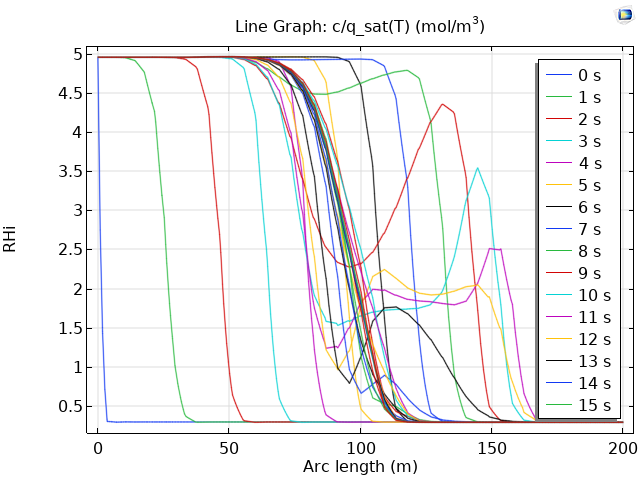
\includegraphics[width=\linewidth]{image1.png}
        \caption{Velocity magnitude}
        \label{fig:comsol_vel0}
    \end{subfigure}
    \hfill
    \begin{subfigure}[b]{0.32\linewidth}
        \centering
        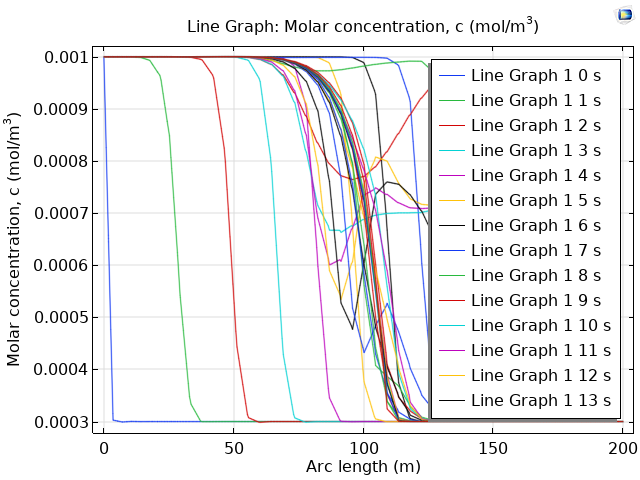
\includegraphics[width=\linewidth]{image2.png}
        \caption{Pressure field}
        \label{fig:comsol_p0}
    \end{subfigure}
    \hfill
    \begin{subfigure}[b]{0.32\linewidth}
        \centering
        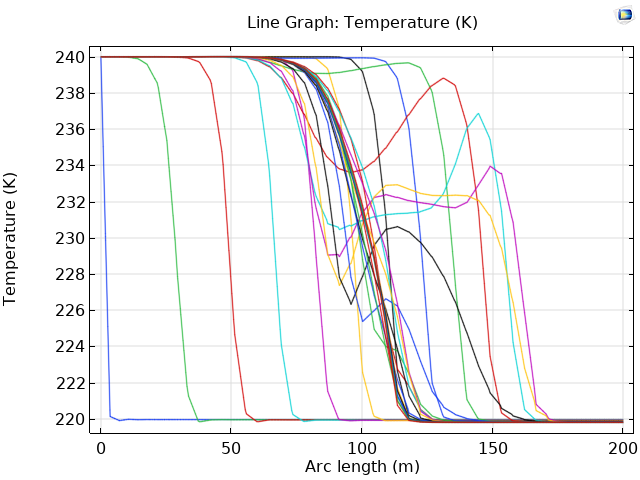
\includegraphics[width=\linewidth]{image3.png}
        \caption{Temperature field}
        \label{fig:comsol_T0}
    \end{subfigure}

    \caption{Resolved COMSOL fields at initialization ($t=0$). The injected plume appears
    as a localized region of elevated velocity and temperature near the inlet, while the
    surrounding flow remains quiescent.}
    \label{fig:comsol_initial}
\end{figure}

\subsection{Time evolution and animated diagnostics}
\label{sec:comsol_animations}

The temporal evolution of the plume is visualized using animated COMSOL exports. Because
animated GIFs cannot be embedded directly in the paper, they are provided as
external links and referenced here:

\paragraph{Flow and thermodynamic evolution (click on links to see very cool and hard worked on GIFs :D)}
\begin{itemize}
\item Velocity field evolution:
\href{run:https://jumpshare.com/share/tsg11veOD7mxcaSBZTff}{\texttt{GIF of Velocity field}}
\item Pressure evolution:
\href{run:https://jumpshare.com/share/jxBsH8VZWwNd2hiq2hHm}{\texttt{GIF of Pressure}}
\item Temperature evolution:
\href{run:https://jumpshare.com/share/e9kANcUsdQniLVNUi2Wr}{\texttt{GIF of Temperature}}

\end{itemize}

\paragraph{Moisture and scalar dilution}
\begin{itemize}
\item Relative humidity over ice (RHi) evolution:
\href{run:https://jumpshare.com/share/vRPYYj6269of2rr7CPT4}{\texttt{GIF of RHi}}
\item Scalar concentration evolution:
\href{https://jumpshare.com/share/vzrJCuPj6kDWgZQWGpS9}{\texttt{GIF of Scalar Concentration}}
\item Combined diagnostic animation:
\href{run:https://jumpshare.com/share/RAviPkzhh5nMQkVhHzew}{\texttt{GIF of combined animation}}
\end{itemize}

These animations show the plume advecting downstream while spreading laterally under the
combined influence of shear and diffusion. The scalar concentration remains confined to
the plume core at early times and progressively decays as dilution dominates.

\subsection{Diagnostic extraction and comparison to the reduced model}
\label{sec:comsol_diagnostics}

To enable quantitative comparison with the reduced-order model, COMSOL outputs are
post-processed to extract diagnostics analogous to those defined in
Section~\ref{sec:matlab_diagnostics}. In particular, cross-stream profiles of $c(y,t)$ at
fixed downstream locations are used to compute an effective plume width,
\begin{equation}
w(t) = \left[
\frac{\int (y-\bar{y})^2 c(y,t)\,dy}{\int c(y,t)\,dy}
\right]^{1/2},
\label{eq:comsol_width}
\end{equation}
from which an effective diffusivity may be inferred using the diffusion scaling
\begin{equation}
K_{\mathrm{eff}}(t) = \frac{w^2(t)-w_0^2}{2t}.
\label{eq:comsol_keff}
\end{equation}

Centerline decay of the scalar concentration provides an additional persistence proxy,
which can be compared directly to the centerline-based lifetime definition used in the
MATLAB model. The agreement between COMSOL-derived $K_{\mathrm{eff}}$ and the parameterized
$K(N,S)$ suppors the effective-diffusivity abstraction. deviations indicate regimes
where shear-driven deformation or non-diffusive transport becomes important.

I, unfortunately, misplaced the Matlab file and could not find the exports in the hundreds of plots generated for this project and hence it has not been shown here. 

\section{Reanalysis-Driven Environmental Diagnostics (ERA5/\texttt{pycontrails})}
\label{sec:pycontrails_era5}

The MATLAB reduced-order model and the COMSOL plume simulations quantify how contrail persistence
depends on three environmental controls, ice supersaturation (RHi), static stability ($N$), and
vertical shear ($S$, when these parameters are treated as tunable inputs. To anchor those
parameter regimes in realistic atmospheric variability, ERA5 reanalysis data were processed using
the \texttt{pycontrails} workflow to compute upper-tropospheric fields relevant to contrail
formation and persistence. 

\subsection{Thermodynamic feasibility: ice supersaturation in space, time, and along-track}
\label{subsec:rhi_results}

Persistent contrails require ambient air to be supersaturated with respect to ice (RHi $>100\%$),
so the first question is whether the upper-tropospheric environment contains sustained
ice-supersaturated regions (ISSRs) in the relevant pressure range. Figure~\ref{fig:rhi_map_track}
shows a representative RHi field at 250~hPa (00Z on 2024-10-10) together with the sampled RHi along
a cruise-level trajectory through western/central Europe. The map reveals that ISSRs are not
uniformly distributed: they occur as narrow, filamentary structures embedded within much larger
sub-saturated areas. This spatial intermittency is consistent with the conceptual picture that
contrail persistence is conditional on passing through specific meteorological features rather
than being guaranteed at cruise altitude.

The along-track RHi time series further illustrates that the aircraft encounters long stretches of
sub-saturated air punctuated by a limited supersaturated segment. In the present trajectory, only
a small fraction of waypoints exceed 100\% RHi (approximately $4\%$), implying that even before
dynamical dilution is considered, persistent-contrail conditions are relatively rare along the
track. This fact provides a direct interpretive link to the MATLAB phase behavior in
Fig.~\ref{fig:matlab_sweeps}--\ref{fig:matlab_phase}: the sharp transition in persistence near
RHi $\approx 100\%$ corresponds, in the reanalysis, to a sparse set of spatiotemporal organized events.

\begin{figure}[t]
    \centering
    \begin{subfigure}[b]{0.49\linewidth}
        \centering
        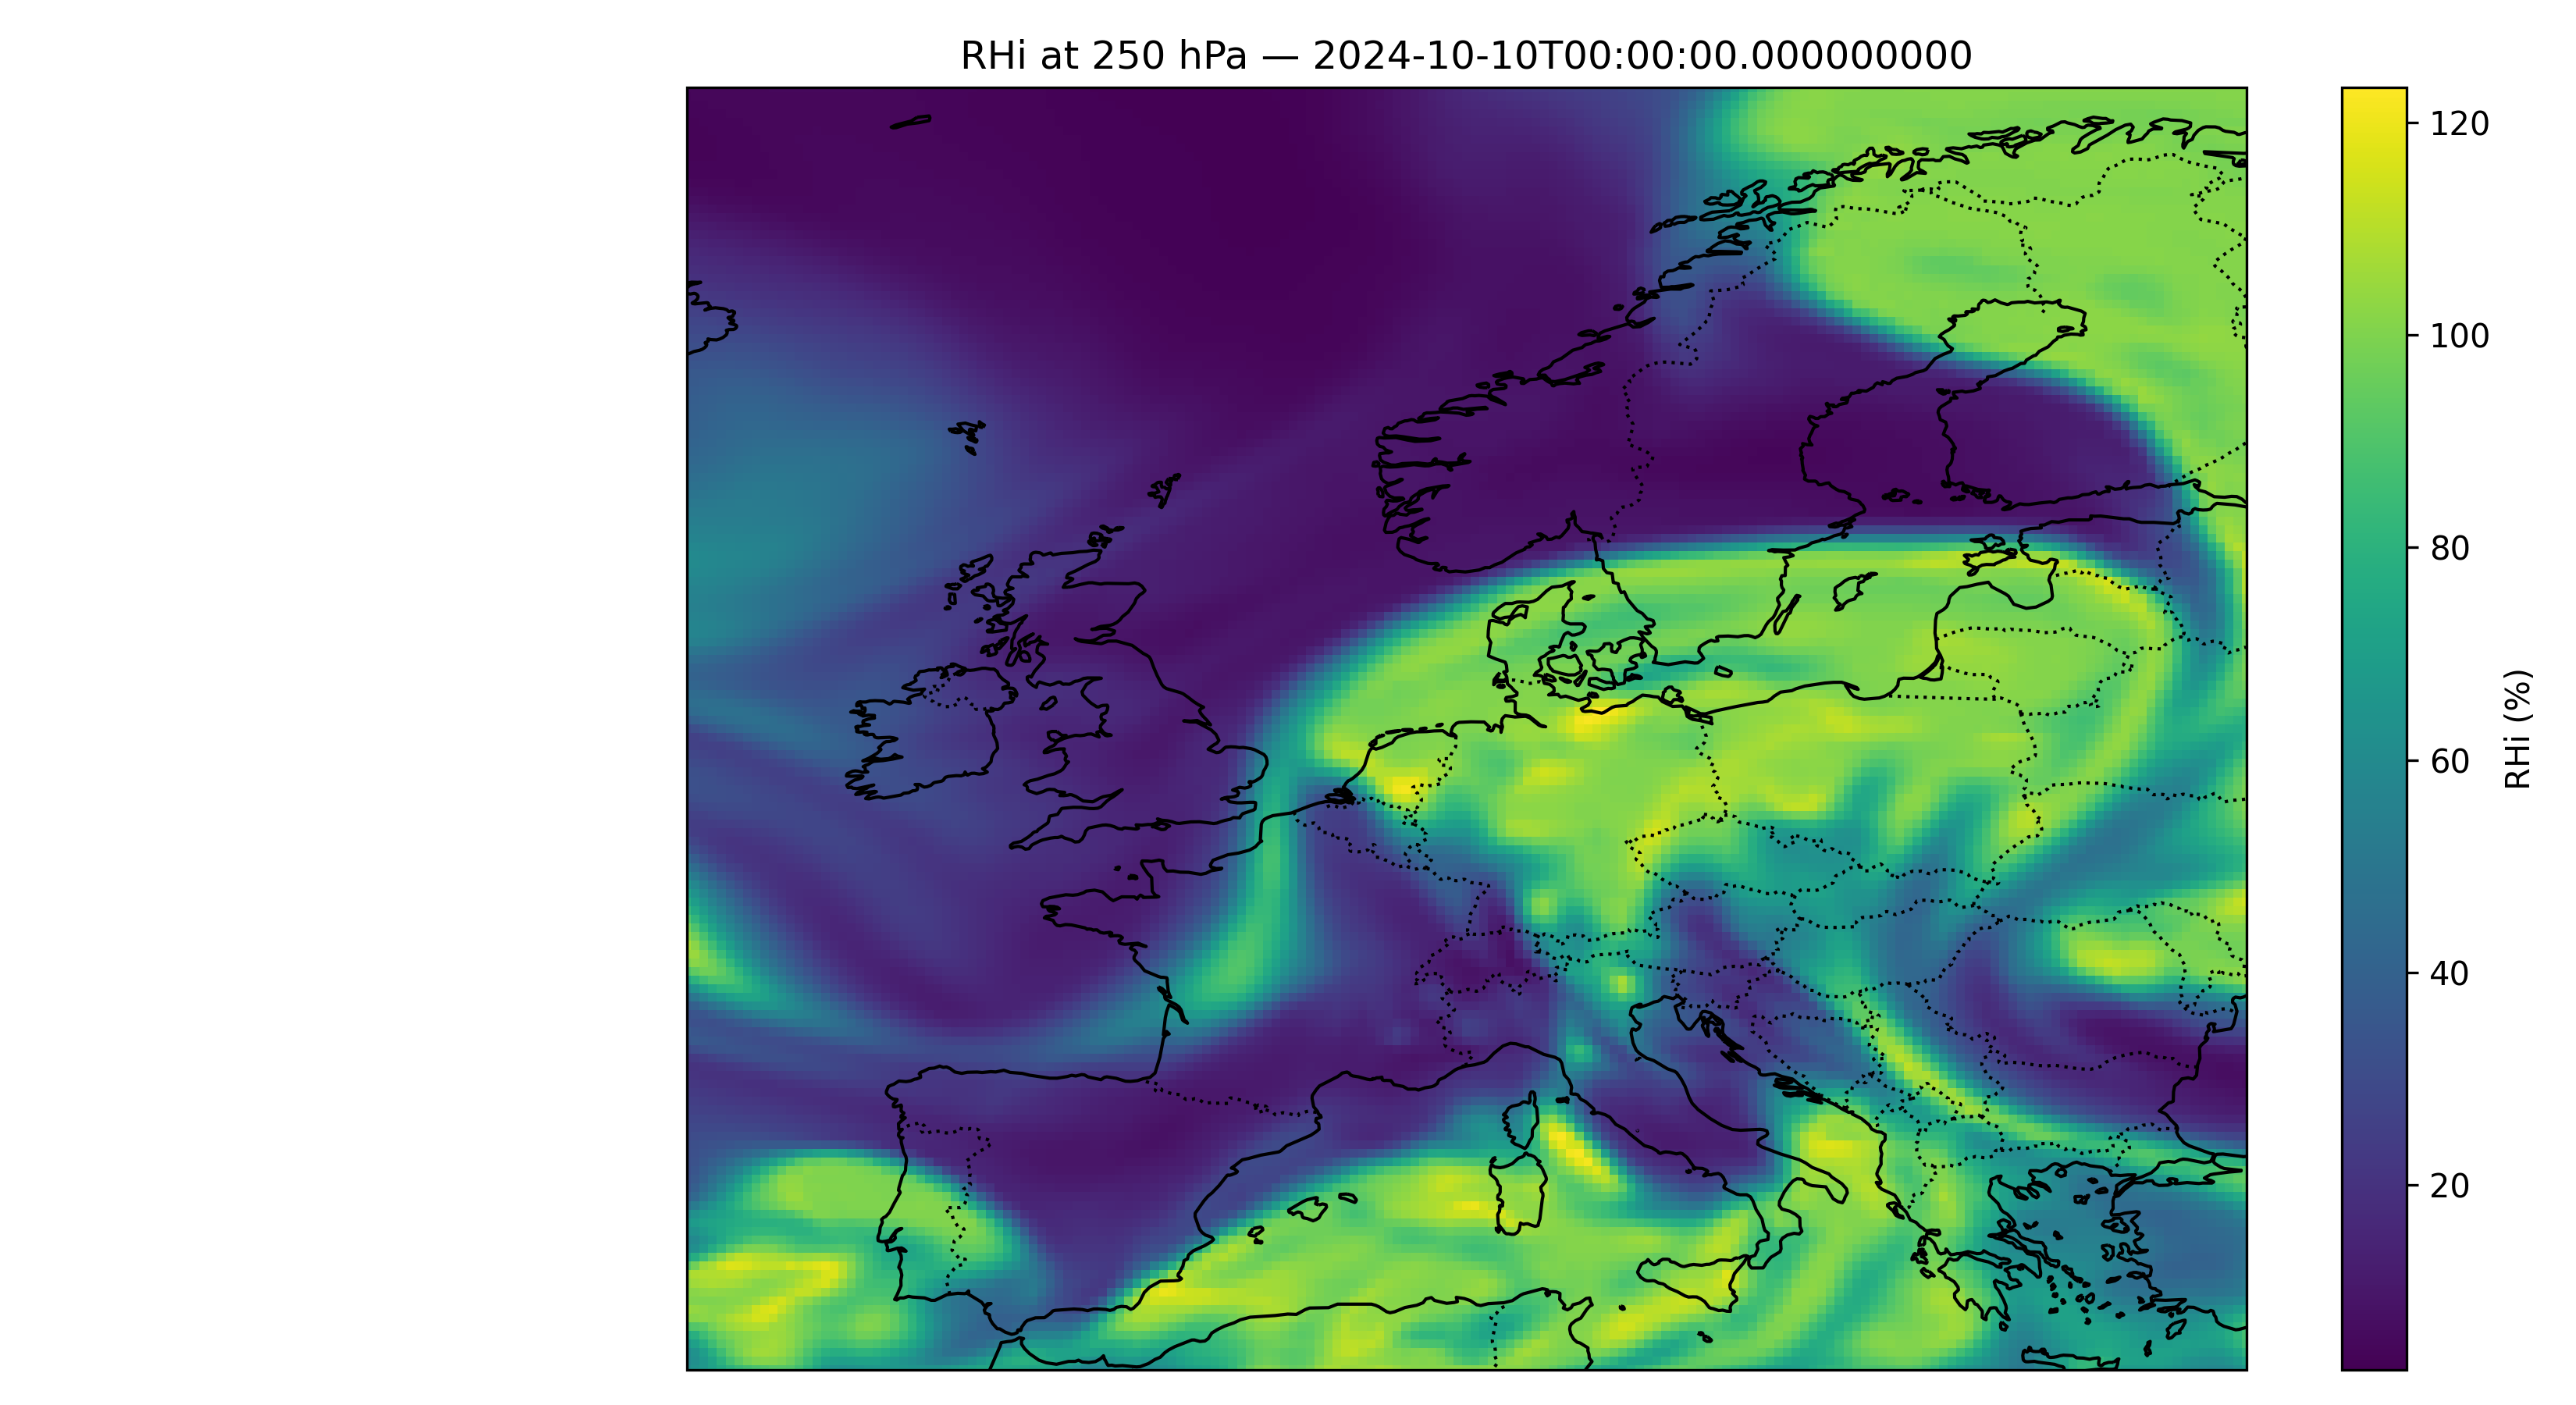
\includegraphics[width=\linewidth]{RHi_250hPa_20241010T00Z.png}
        \caption{RHi at 250~hPa (00Z, 2024-10-10)}
        \label{fig:rhi_map_250}
    \end{subfigure}
    \hfill
    \begin{subfigure}[b]{0.49\linewidth}
        \centering
        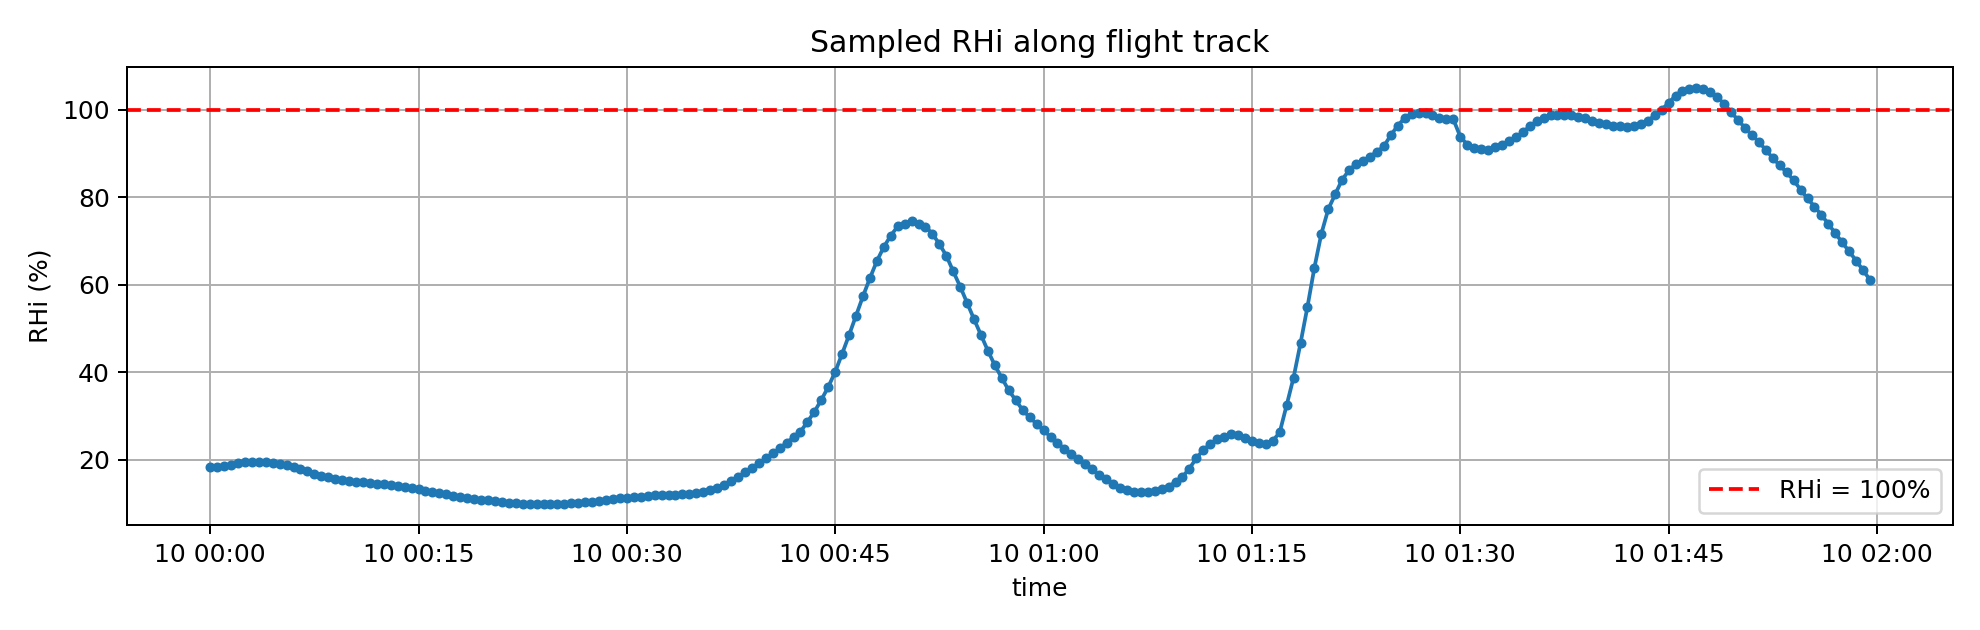
\includegraphics[width=\linewidth]{flight_RHi_timeseries.png}
        \caption{Sampled RHi along flight trajectory}
        \label{fig:rhi_track}
    \end{subfigure}
    \caption{Ice supersaturation in the upper troposphere from ERA5/\texttt{pycontrails}.
    (a) A representative RHi field at 250~hPa exhibits spatially intermittent ISSRs (RHi$>100\%$).
    (b) Along-track sampling shows extended sub-saturated segments and a limited supersaturated
    interval, motivating a persistence framework that is conditional on thermodynamic feasibility.}
    \label{fig:rhi_map_track}
\end{figure}

To contextualize the single-track sampling, Europe-wide statistics were computed over the full
domain and all available analysis times. Figure~\ref{fig:eu_stats} summarizes the areal prevalence
of ISSRs and the distribution of RHi at multiple pressure levels. The area fraction with
RHi$>100\%$ varies systematically with both time and altitude, typically spanning
$\mathcal{O}(5\text{--}20\%)$ depending on level. Higher levels (e.g.\ 300--250~hPa) generally show
larger supersaturated fractions than lower levels (225--200~hPa), consistent with colder ambient
temperatures and upper-level dynamical forcing. The pooled histograms display a strongly skewed
RHi distribution with a long tail beyond saturation, reinforcing that ISSRs represent the
high-humidity tail of upper-tropospheric variability rather than the mean state.

\begin{figure}[t]
    \centering
    \begin{subfigure}[b]{0.49\linewidth}
        \centering
        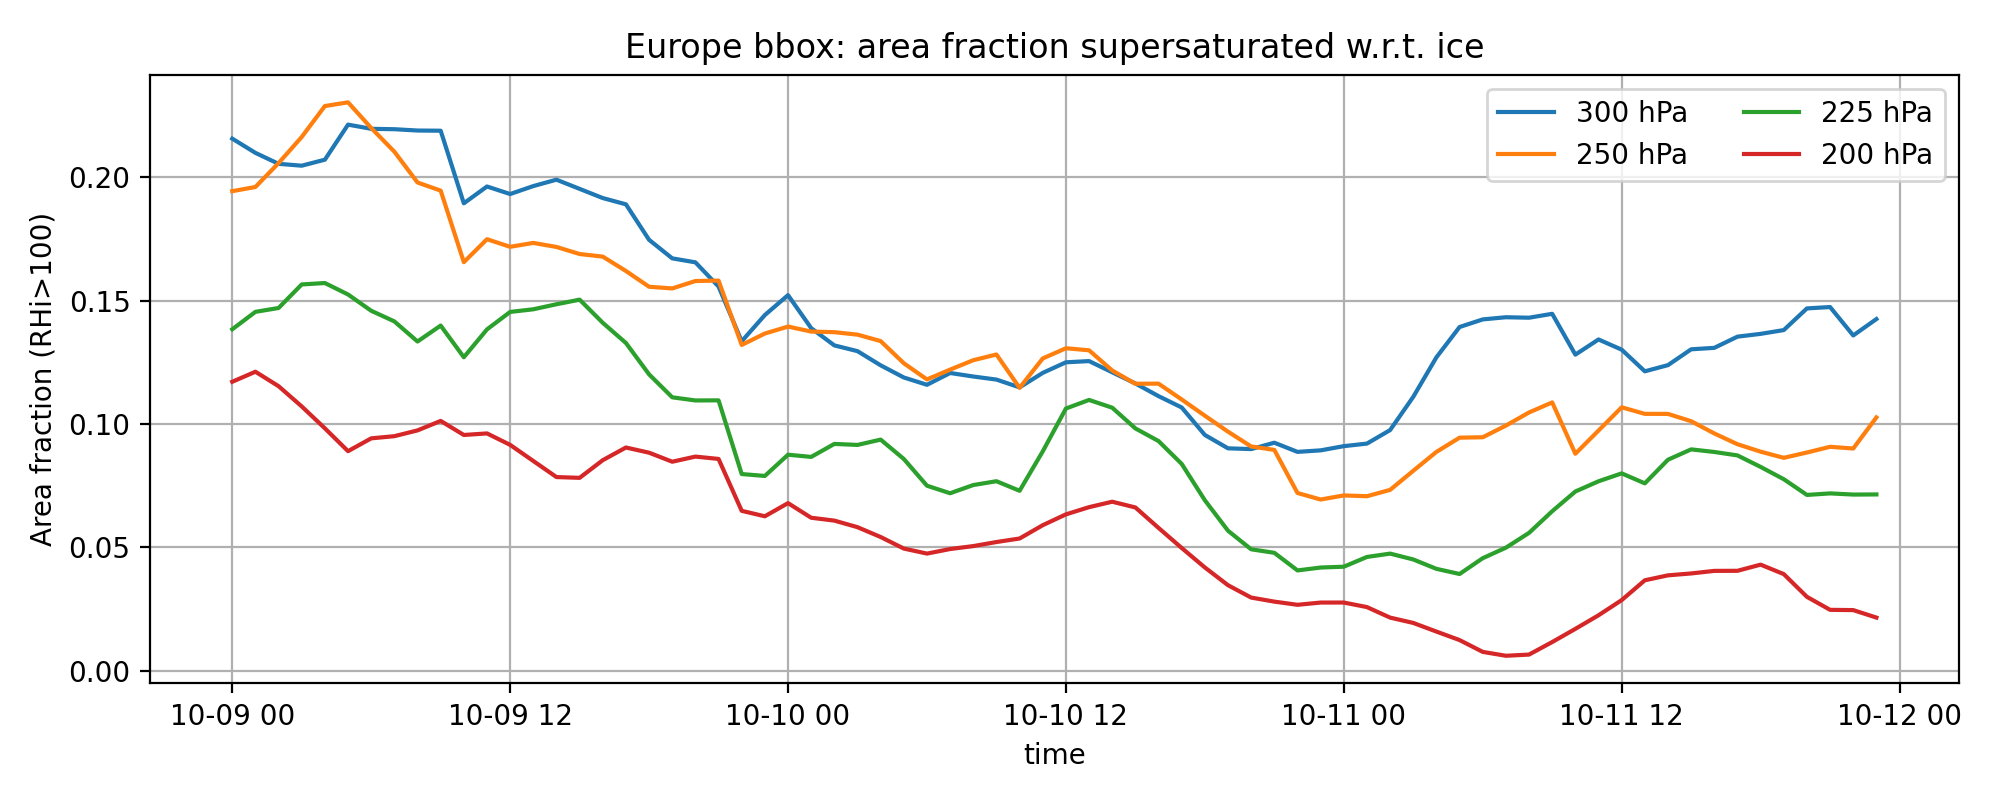
\includegraphics[width=\linewidth]{area_fraction_RHi_gt100.png}
        \caption{Area fraction (RHi$>100\%$) vs time}
        \label{fig:area_fraction}
    \end{subfigure}
    \hfill
    \begin{subfigure}[b]{0.49\linewidth}
        \centering
        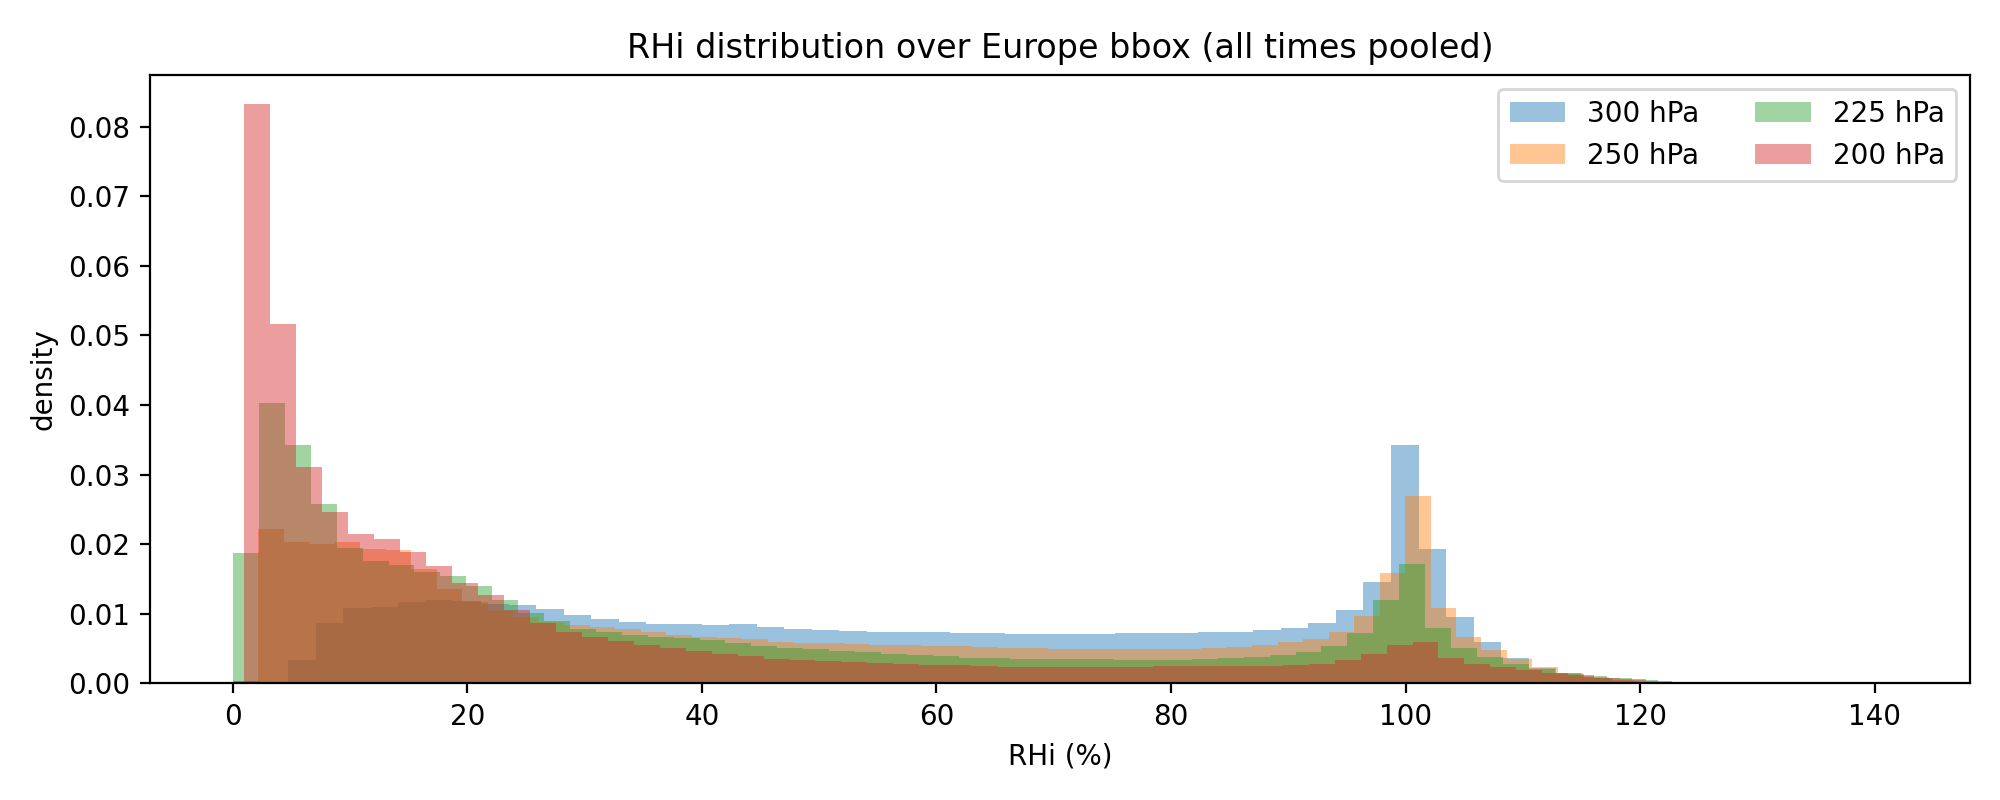
\includegraphics[width=\linewidth]{RHi_hist_by_level.png}
        \caption{RHi distribution (all times pooled)}
        \label{fig:rhi_hist}
    \end{subfigure}
    \caption{Regional context for ice supersaturation over Europe.
    (a) The fraction of the domain that is ice-supersaturated varies with synoptic evolution and
    altitude, indicating that persistence potential is meteorology-dependent.
    (b) Pooled histograms show that supersaturation occurs in the tail of a skewed distribution,
    consistent with the limited along-track supersaturation fraction.}
    \label{fig:eu_stats}
\end{figure}

\subsection{Dynamical controls: stability and shear as reanalysis analogues of plume transport}
\label{subsec:n2_shear_results}

While ISSRs determine whether ice growth is thermodynamically possible, the persistence lifetime
and morphology depend on the rate at which the plume mixes and deforms. In the MATLAB model,
these effects were encoded through an effective diffusivity $K(N,S)$ (Eq.~\eqref{eq:K}), while the
COMSOL simulations resolved advection--diffusion and shear-driven deformation explicitly. ERA5
provides the corresponding dynamical controls via stability and vertical shear diagnostics.

Potential temperature was computed as $\theta = T(p_0/p)^{R/c_p}$, and the Brunt--V\"ais\"al\"a
frequency squared was obtained from \cite{Holton2013}
\begin{equation}
    N^2 = \frac{g}{\theta}\frac{\partial \theta}{\partial z}.
\end{equation}
using finite differences in the vertical after converting geopotential to geometric height
$z_{\mathrm{geo}}=z/g$. Vertical shear was computed from \cite{Holton2013}
\begin{equation}
    S = \sqrt{\left(\frac{\partial u}{\partial z}\right)^2 + \left(\frac{\partial v}{\partial z}\right)^2}.
\end{equation}
Figures~\ref{fig:n2_shear_maps} show representative maps of $N^2$ and $S$ at 250~hPa. The $N^2$
field exhibits smooth, synoptic-scale structure consistent with large-scale stratification, while
the shear field shows sharper filaments associated with jets and frontal zones. The magnitudes
obtained are physically reasonable for the upper troposphere (here, $N^2 \sim 10^{-5}$--$10^{-4}
\,\mathrm{s^{-2}}$ and $S \sim 10^{-3}$--$10^{-2}\,\mathrm{s^{-1}}$), placing the reanalysis
environment squarely within the sweep ranges explored in MATLAB and the deformation regimes
represented in COMSOL.

\begin{figure}[t]
    \centering
    \begin{subfigure}[b]{0.49\linewidth}
        \centering
        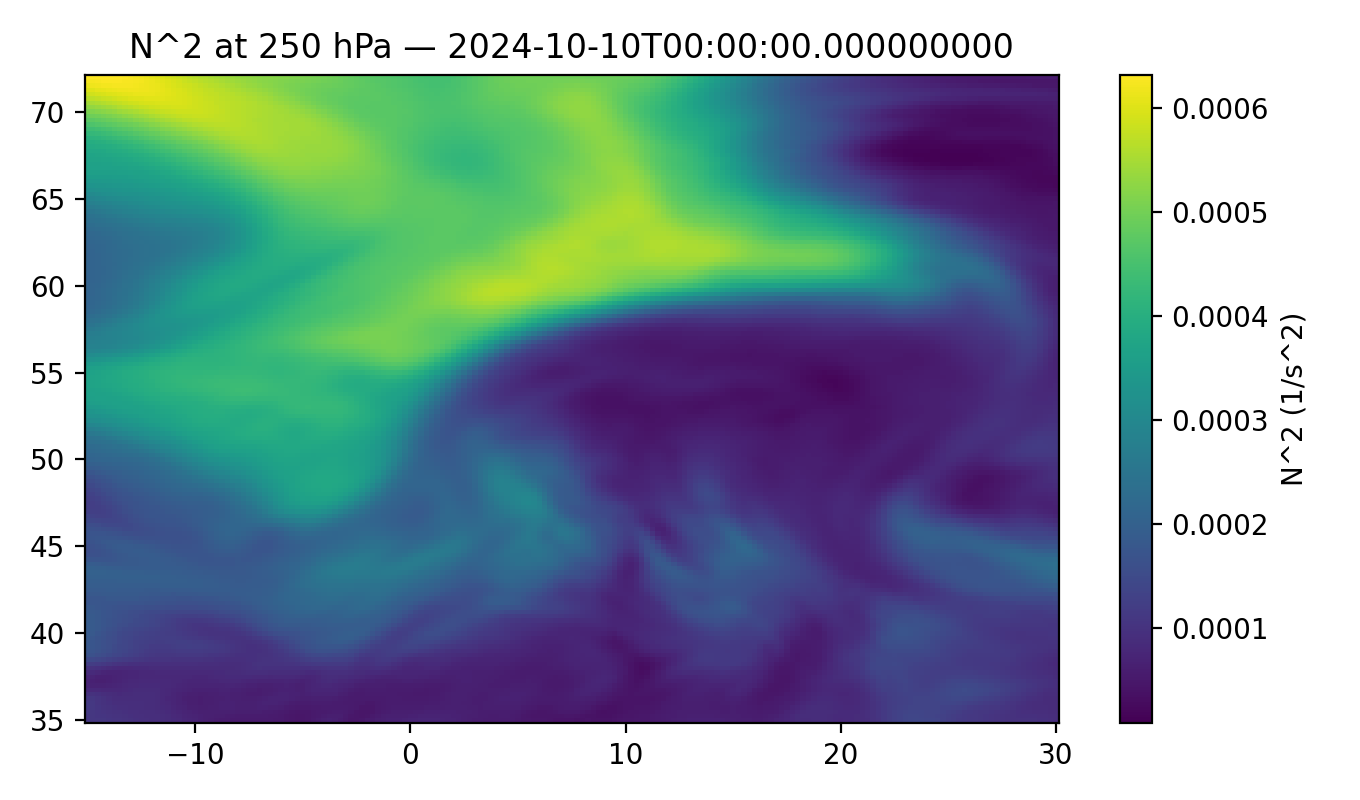
\includegraphics[width=\linewidth]{N2_250hPa_fixed.png}
        \caption{$N^2$ at 250~hPa}
        \label{fig:n2_map}
    \end{subfigure}
    \hfill
    \begin{subfigure}[b]{0.49\linewidth}
        \centering
        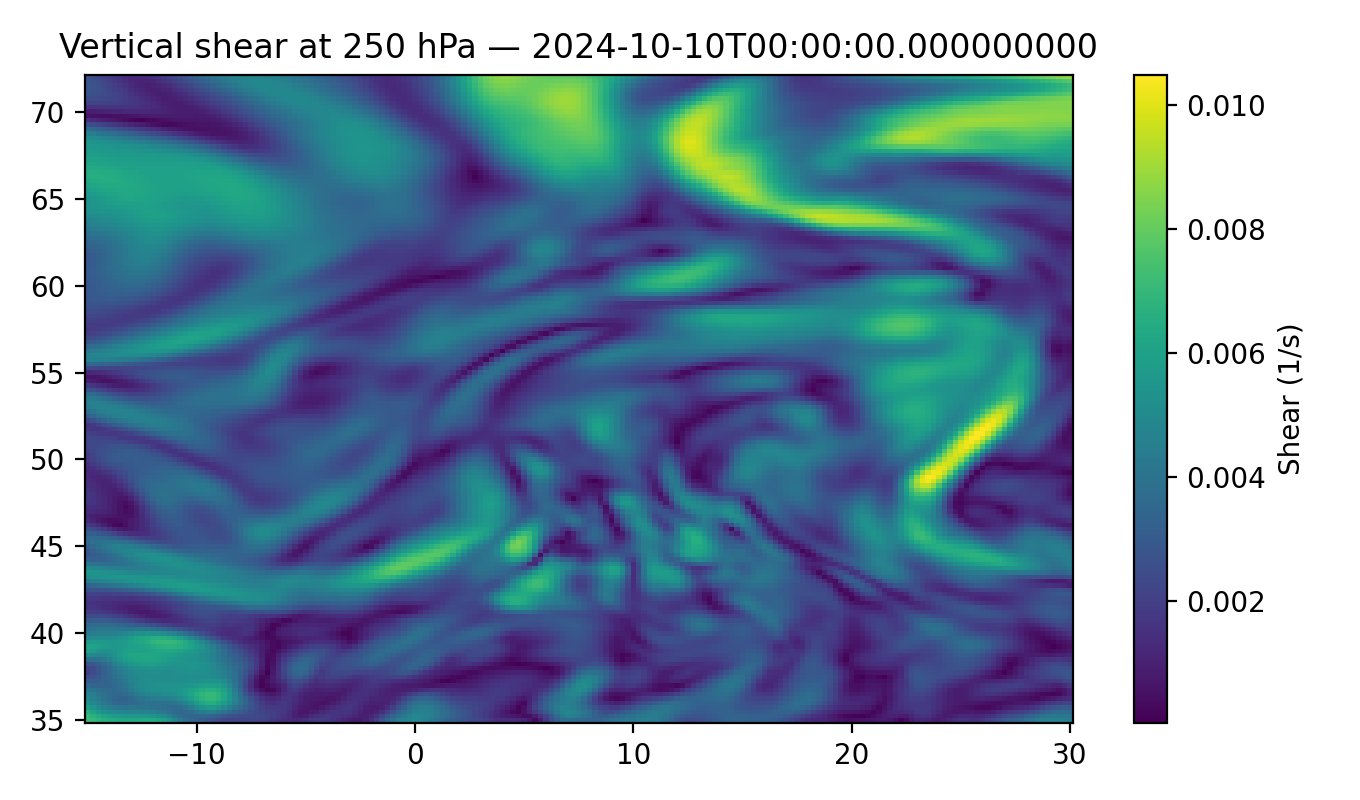
\includegraphics[width=\linewidth]{Shear_250hPa_fixed.png}
        \caption{Vertical shear at 250~hPa}
        \label{fig:shear_map}
    \end{subfigure}
    \caption{Dynamical controls on contrail persistence from ERA5.
    Static stability ($N^2$) varies smoothly on synoptic scales, while vertical shear exhibits
    sharper gradients associated with strong-flow features. These diagnostics provide
    meteorologically grounded analogues for the transport/dilution controls represented by
    $K(N,S)$ in the MATLAB model and resolved explicitly in COMSOL.}
    \label{fig:n2_shear_maps}
\end{figure}

\subsection{A unified persistence indicator and connection to plume-scale results}
\label{subsec:persistence_indicator}

To connect the reanalysis environment to the reduced-order persistence picture, a compact
persistence indicator was constructed along the trajectory using three ingredients: (i) humidity
availability (RHi), (ii) stratification (via $N^2$), and (iii) deformation/mixing potential (via
shear $S$). A ``raw'' score was first defined as a weighted sum of normalized components,
\begin{equation}
    \mathcal{P}_{\mathrm{raw}}
    = w_{\mathrm{RHi}}\;\widetilde{\mathrm{RHi}}
    + w_{N}\;\widetilde{N^2}
    + w_{S}\;\left(1-\widetilde{S}\right),
    \qquad
    w_{\mathrm{RHi}}+w_N+w_S=1,
\end{equation}
where tildes denote robust normalization to $[0,1]$ using percentile scaling. The factor
$1-\widetilde{S}$ encodes the expectation that stronger shear accelerates plume deformation and
dilution, reducing persistence of a coherent core. This representation mirrors the MATLAB closure
(Eq.~\eqref{eq:K}) in which increasing shear increases effective mixing, and it is consistent with
COMSOL behavior in which shear-driven stretching enhances dilution rates along the cross-plume
direction.

Figure~\ref{fig:raw_score_scatter} shows the relationship between vertical shear and
$\mathcal{P}_{\mathrm{raw}}$, colored by RHi. Two features are prominent. First, there is a clear
anticorrelation between shear and the raw score: high shear environments systematically correspond
to lower persistence favorability. Second, humidity modulates this relationship: high-RHi points
populate the upper envelope of $\mathcal{P}_{\mathrm{raw}}$, while low-RHi points cluster at lower
scores. This joint dependence provides a reanalysis analogue of the MATLAB regime behavior: the
MATLAB sweeps show that near-threshold humidity is particularly sensitive to dynamical dilution,
and the reanalysis scatter exhibits that the highest persistence favorability occurs when both
humidity and dynamical conditions align.

\begin{figure}[t]
    \centering
    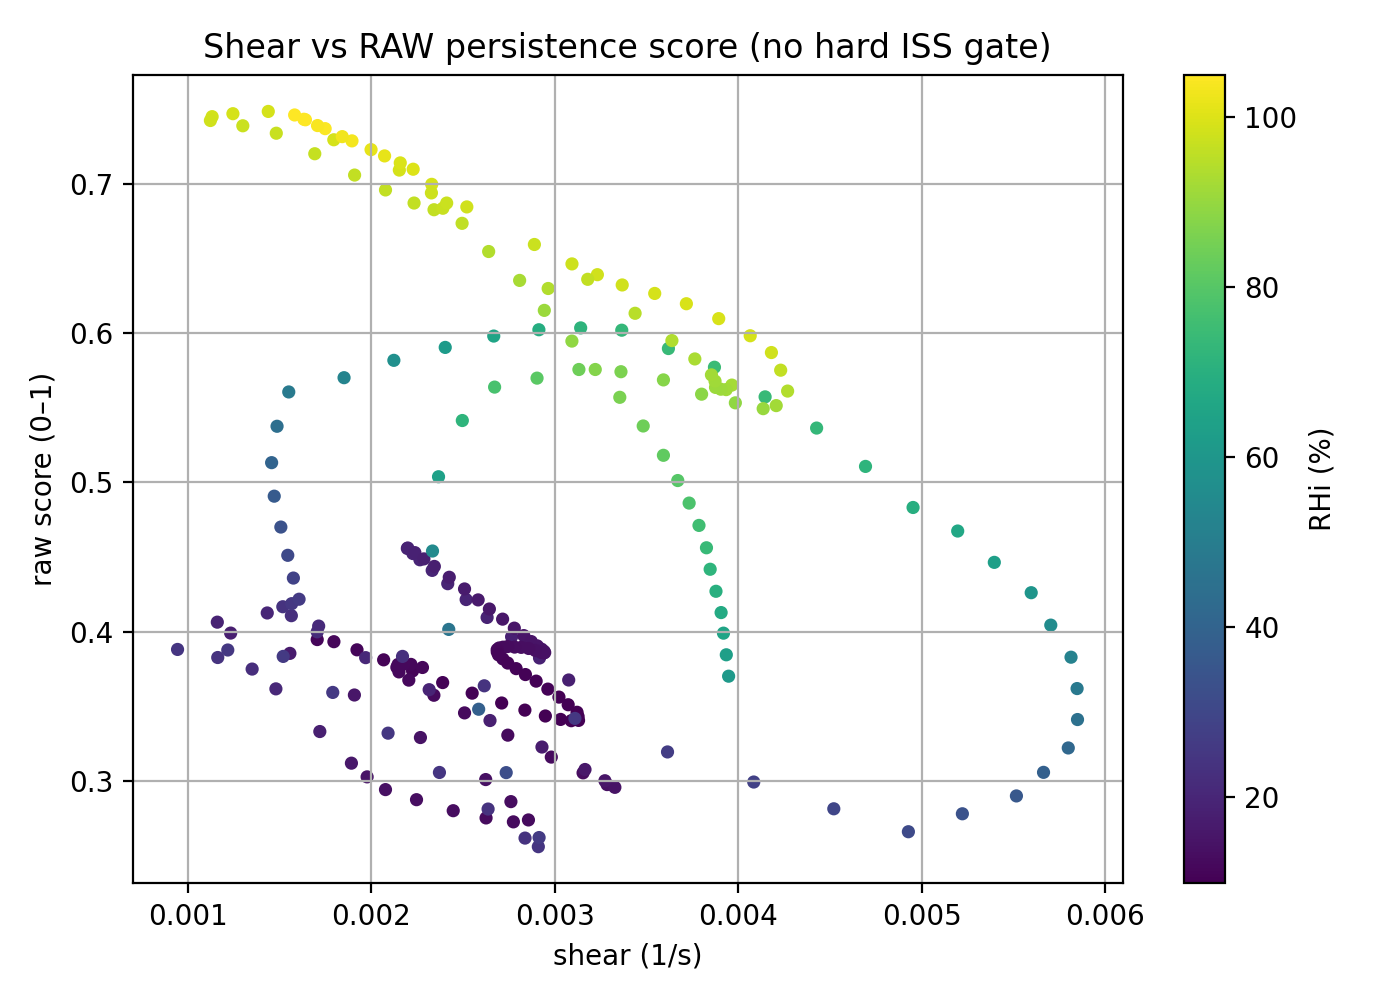
\includegraphics[width=0.72\linewidth]{scatter_shear_vs_score_RAW_colored_RHi.png}
    \caption{Relationship between vertical shear and a raw persistence favorability score along the
    flight, colored by RHi. Higher shear is associated with lower persistence favorability, while
    higher humidity shifts the score upward across the shear range. This mirrors the MATLAB
    sensitivity of persistence to shear under marginal humidity and is consistent with shear-driven
    deformation/dilution mechanisms resolved in COMSOL.}
    \label{fig:raw_score_scatter}
\end{figure}

Because persistent contrails require (at minimum) near-ice-saturated conditions, a moisture gating
factor was introduced to softly enforce thermodynamic feasibility while avoiding an overly brittle
binary threshold. The gating function was chosen as a sigmoid centered at RHi$=100\%$,
\begin{equation}
    \mathcal{G}(\mathrm{RHi})
    = \left(1+\exp\left[-k\left(\mathrm{RHi}-100\right)\right]\right)^{-1},
\end{equation}
with $k$ controlling the sharpness of transition. The final soft-gated indicator is
$\mathcal{P}_{\mathrm{soft}}=\mathcal{P}_{\mathrm{raw}}\mathcal{G}(\mathrm{RHi})$.
Figure~\ref{fig:soft_gate} shows the gating curve and the resulting shear--score relationship. As
expected, the soft-gated score collapses toward zero in strongly sub-saturated air and highlights
a small subset of waypoints where persistence is plausible. In the present trajectory, only
$\approx 4\%$ of waypoints are ice-supersaturated, which explains the sparse set of elevated
$\mathcal{P}_{\mathrm{soft}}$ values. This sparsity is not a numerical artifact. It is a direct
expression of the thermodynamic threshold that also appears in the MATLAB lifetime sweeps.

\begin{figure}[t]
    \centering
    \begin{subfigure}[b]{0.49\linewidth}
        \centering
        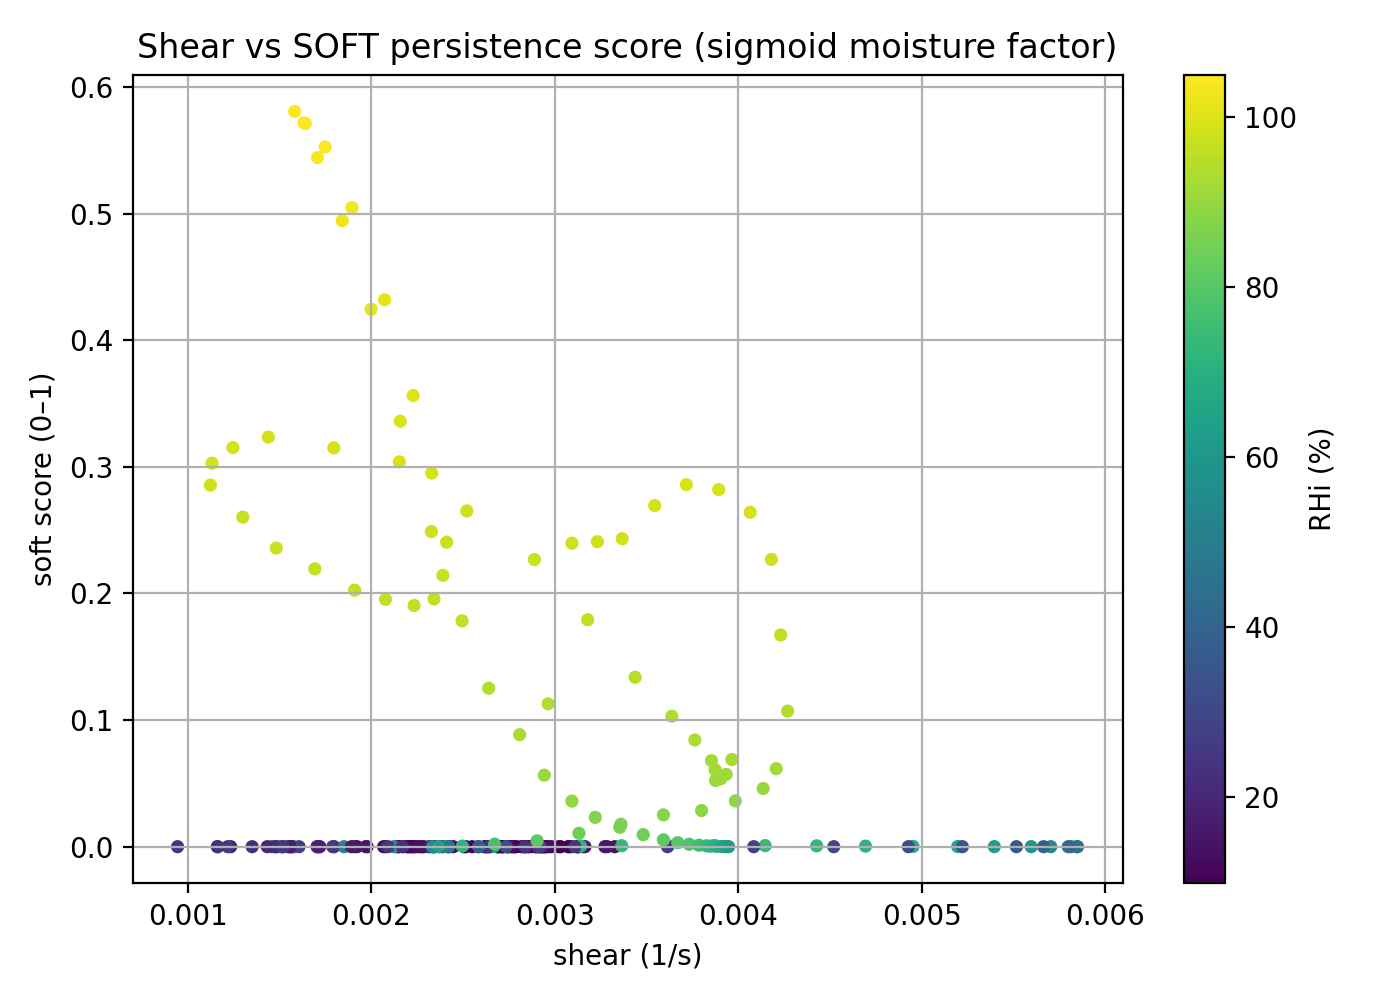
\includegraphics[width=\linewidth]{scatter_shear_vs_score_SOFT_colored_RHi.png}
        \caption{Shear vs soft-gated score $\mathcal{P}_{\mathrm{soft}}$}
        \label{fig:soft_score_scatter}
    \end{subfigure}
    \hfill
    \begin{subfigure}[b]{0.49\linewidth}
        \centering
        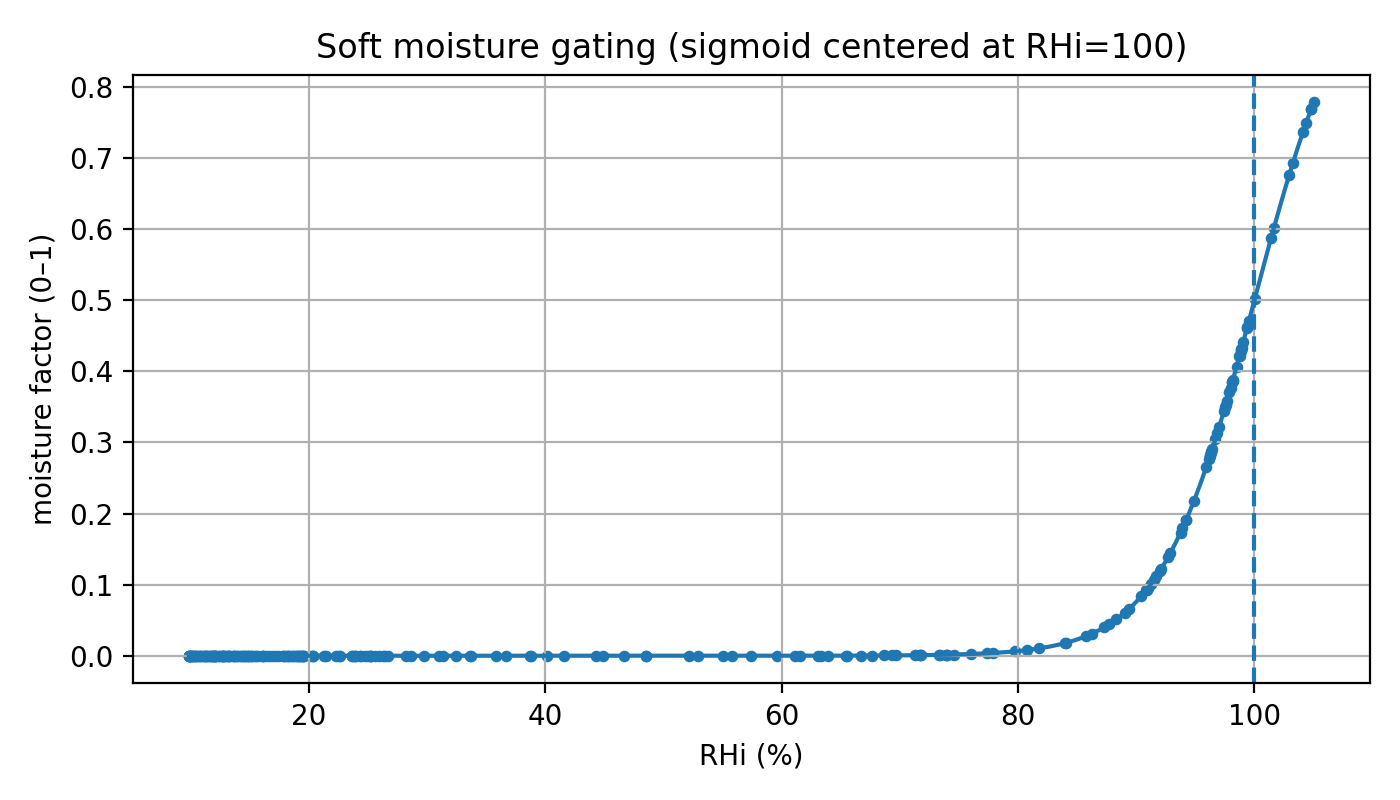
\includegraphics[width=\linewidth]{moisture_factor_sigmoid.png}
        \caption{Moisture gating $\mathcal{G}(\mathrm{RHi})$}
        \label{fig:moisture_sigmoid}
    \end{subfigure}
    \caption{Soft enforcement of thermodynamic feasibility for persistence.
    A sigmoid gating centered at RHi$=100\%$ suppresses persistence in strongly sub-saturated air
    while allowing continuous transitions near the threshold. The resulting $\mathcal{P}_{\mathrm{soft}}$
    highlights a small set of waypoints as plausibly persistent, consistent with the limited ISS
    prevalence in both the along-track sampling and the regional statistics.}
    \label{fig:soft_gate}
\end{figure}

\subsection{Synthesis across scales: interpreting ERA5 diagnostics through MATLAB and COMSOL}
\label{subsec:multiscale_link}

The combined ERA5/\texttt{pycontrails} diagnostics provide a consistent bridge between the
idealized parameter sweeps (MATLAB) and the resolved transport physics (COMSOL). The MATLAB model
predicts a sharp persistence transition near ice saturation and systematic modulation by shear and
stability when humidity is marginal. The reanalysis results show exactly the environmental
structure required for that picture: ISSRs occupy a small, organized portion of the domain (and a
small fraction of the flight), while shear and stability vary across the same order-of-magnitude
ranges used in the reduced model. COMSOL, in turn, supplies mechanistic support for interpreting
shear as a deformation-driven dilution pathway, which rationalizes the anticorrelation between
shear and persistence favorability seen in the raw-score scatter.

Overall, the multiscale results support a two-part persistence criterion: contrails are
thermodynamically feasible only within localized ISSRs, and their subsequent persistence is
regulated by the competition between stabilizing stratification and shear-driven deformation and
mixing. This framing provides a physically grounded pathway for using reanalysis meteorology to
interpret and constrain plume-scale persistence models without relying on satellite detection or
case-by-case manual classification.
\section{Summary and Conclusions}
\label{sec:conclusions}

\subsection{Hypothesis check}
This project began with the hypothesis that contrail persistence is primarily gated by
\textbf{ice supersaturation} (RHi), with \textbf{dynamical dilution} set by stability ($N$) and
vertical shear ($S$) modulating lifetime once conditions are near threshold. Across the three
modeling tiers developed here, the results support that hypothesis:

\begin{itemize}
    \item \textbf{Thermodynamic control (RHi) is the dominant gate.}
    The MATLAB reduced-order model shows a sharp transition in the persistence proxy
    $\tau_{\mathrm{persist}}$ near RHi $\approx 100\%$, consistent with the physical requirement
    that ice cannot be maintained in subsaturated air. The ERA5/\texttt{pycontrails} diagnostics
    show that ice-supersaturated regions (ISSRs) are spatially intermittent and occupy a limited
    fraction of the domain/trajectory, meaning that persistence-capable conditions are rare in
    both space and time.
    \item \textbf{Shear and stability modulate persistence under marginal humidity.}
    When RHi is near (but below) saturation, the MATLAB sweeps demonstrate systematic sensitivity
    of lifetime to the effective mixing control $K(N,S)$: stronger shear shortens lifetime via
    enhanced dilution, while stability changes mixing rates and therefore the decay of the plume
    core. In the reanalysis-based indicator, higher shear is associated with lower persistence
    favorability, consistent with the same mechanism.
    \item \textbf{Mechanistic interpretation is consistent across tiers.}
    COMSOL resolves the spatial plume deformation and advection--diffusion physics that are
    parameterized in the reduced model. The resulting picture is coherent: \emph{RHi determines
    whether persistence is feasible at all}, and \emph{transport controls determine how rapidly the
    plume core dilutes once feasible}.
\end{itemize}

\subsection{What we learned about the question}
The central question was: \emph{How do RHi, static stability, and vertical wind shear jointly
control contrail plume persistence?} The main takeaways are:

\begin{enumerate}
    \item \textbf{Persistence is a two-part condition: feasibility + survivability.}
    Feasibility is set by the thermodynamic threshold (RHi near or above $100\%$), while survivability
    depends on how quickly mixing reduces centerline concentration/ice proxy below a detectability
    or “persistence” threshold.
    \item \textbf{Near-threshold regimes are the most sensitive.}
    The strongest dynamical sensitivity occurs when RHi is close to saturation, where modest changes
    in mixing rates can shift the system between short-lived and persistent behavior (seen clearly in
    MATLAB phase behavior and in the reanalysis scatter/soft-gated score).
    \item \textbf{A practical interpretation for meteorology-driven prediction emerges.}
    In reanalysis space, ISSRs identify where persistence is possible. Then shear/stability diagnostics
    provide a physically interpretable ordering of “more” vs “less” persistence-favorable environments.
\end{enumerate}

\subsection{Limitations}
The framework is intentionally hierarchical and therefore simplified:
(i) the MATLAB microphysics is bulk/parametric rather than particle-resolved,
(ii) COMSOL is 2D and does not represent full 3D turbulence/microphysics coupling, and
(iii) ERA5 provides resolved-scale meteorology but not subgrid supersaturation variability.

% ============================================================
% SECTION 6 — Future Work
% ============================================================

\section{Future Work}
\label{sec:future}

Several follow-up directions would materially strengthen the answer to the persistence question and
move the framework closer to predictive capability:

\begin{enumerate}
    \item \textbf{Upgrade the microphysics in the reduced model.}
    Replace the bulk piecewise growth/decay closure with a minimal but physical scheme
    (e.g., ice crystal number/mass evolution with temperature-dependent saturation vapor pressure,
    deposition/sublimation kinetics, and sedimentation). This would allow the RHi threshold behavior
    to emerge from physics rather than being imposed.
    \item \textbf{Calibrate $K(N,S)$ using COMSOL-inferred transport metrics.}
    Use COMSOL time-dependent plume widths $w(t)$ to infer $K_{\mathrm{eff}}(t)$ and fit a stability/shear
    closure that better represents shear-driven stretching versus purely diffusive spreading.
    This would tighten the link between the reduced model and resolved dynamics.
    \item \textbf{Add radiative relevance metrics.}
    Extend “persistence” beyond a centerline threshold by coupling to simple optical depth or ice water
    path proxies, enabling a clearer connection to radiative forcing rather than lifetime alone.
    \item \textbf{Expand the meteorological sampling.}
    Repeat the ERA5/\texttt{pycontrails} workflow across many days/seasons and multiple flight tracks
    to quantify how often the atmosphere occupies different regions of the $(\mathrm{RHi},N,S)$ phase space,
    and to identify regimes associated with jets/frontal zones versus quiescent conditions.
    \item \textbf{Validation against observations and/or higher-fidelity models.}
    Compare predicted persistence regimes against satellite-based contrail datasets or case-study
    observations, and (if available) benchmark against LES contrail studies to quantify biases from 2D
    transport assumptions and simplified microphysics.
\end{enumerate}

% ============================================================
% SECTION — Code Availability
% ============================================================

\section{Code Availability}
\label{sec:code}

All custom code used in this study is documented below to support transparency and
reproducibility.

\subsection{Python (ERA5 and \texttt{pycontrails})}

All Python-based reanalysis processing, trajectory sampling, and diagnostic plotting
was performed in a Google Colab notebook, which includes all dependencies, data access
instructions, and executable cells.

\noindent
\textbf{Google Colab notebook:}  
\url{https://colab.research.google.com/drive/1f880jXfbDlPuoSE94C86UB5B2F6O0TLD#scrollTo=bTiiFLwMhFk9&uniqifi}

\subsection{MATLAB reduced-order plume model}

The reduced-order plume model described in Section~\ref{sec:matlab_model} was implemented
entirely in MATLAB. The full source code used to generate all MATLAB figures and results
is provided below.

\begin{verbatim}
% ============================================================
% contrail_plume_model.m
% Reduced-order 1D contrail plume model


clear; close all; clc;

% Example environmental values for a basic sweep (coarse table)
RHi_vals_basic = [90, 100, 110];      % Relative humidity w.r.t. ice (%)
N_vals_basic   = [0.005, 0.010];      % Brunt–Väisälä frequency (s^-1)
S_vals_basic   = [0.002, 0.010];      % Vertical wind shear (s^-1)

% Numerical / physical parameters grouped in a struct
params = struct();
params.Ly            = 200;      % domain width in meters (cross-plume)
params.Ny            = 201;      % number of grid points
params.t_end         = 1800;     % max simulation time [s]
params.CFL           = 0.45;     % CFL safety factor for diffusion

params.qi0_center    = 1e-5;     % initial centerline ice mixing ratio [kg/kg]
params.plume_sigma_y = 15;       % initial plume half-width [m]

params.K0            = 1.0;      % base diffusivity [m^2/s]
params.N_ref         = 0.01;     % reference N for scaling [s^-1]
params.S_ref         = 0.01;     % reference shear for scaling [s^-1]
params.kN            = 2.0;      % sensitivity of K to stability
params.kS            = 2.0;      % sensitivity of K to shear

% Microphysics: decay if RHi < 100%, weak growth if RHi > 100%
params.tau_micro     = 90;       % microphysical e-folding time [s]
params.threshold_frac= 0.20;     % lifetime: centerline < 20% of initial

params.T_env         = 220;      % K (not used directly here)

% Lifetime threshold for "persistent" classification (e.g. 10 minutes)
tau_persist_thresh   = 600;      % [s]


fprintf('=== Basic parameter sweep: lifetime vs (RHi, N, S) ===\n');
fprintf('RHi(%%)\tN (s^-1)\tS (s^-1)\tLifetime (s)\n');

for iR = 1:numel(RHi_vals_basic)
    for iN = 1:numel(N_vals_basic)
        for iS = 1:numel(S_vals_basic)
            RHi = RHi_vals_basic(iR);
            N   = N_vals_basic(iN);
            S   = S_vals_basic(iS);

            result = simulate_contrail_1D(RHi, N, S, params);
            tau_persist = result.tau_persist;

            fprintf('%5.0f\t%7.4f\t%7.4f\t%8.1f\n', RHi, N, S, tau_persist);
        end
    end
end


% ---------- Sweep in RHi (holding N, S fixed) ----------
RHi_vec = 80:2:130;
N_fixed_for_RHi = 0.008;
S_fixed_for_RHi = 0.005;

tau_RHi = zeros(size(RHi_vec));

for i = 1:numel(RHi_vec)
    result = simulate_contrail_1D(RHi_vec(i), N_fixed_for_RHi, S_fixed_for_RHi, params);
    tau_RHi(i) = result.tau_persist;
end

figure;
plot(RHi_vec, tau_RHi, 'o-');
xlabel('RHi (%)');
ylabel('Lifetime \tau_{persist} (s)');
title(sprintf('Contrail lifetime vs RHi (N = %.3f s^{-1}, S = %.3f s^{-1})', ...
    N_fixed_for_RHi, S_fixed_for_RHi));
grid on;

% ---------- Sweep in N (holding RHi, S fixed) ----------
% Use a *marginal* humidity so N actually matters (not fully persistent)
N_vec = 0.003:0.001:0.015;
RHi_fixed_for_N = 95;      % < 100%, so some cases decay
S_fixed_for_N   = 0.005;

tau_N = zeros(size(N_vec));

for i = 1:numel(N_vec)
    result = simulate_contrail_1D(RHi_fixed_for_N, N_vec(i), S_fixed_for_N, params);
    tau_N(i) = result.tau_persist;
end

figure;
plot(N_vec, tau_N, 'o-');
xlabel('N (s^{-1})');
ylabel('Lifetime \tau_{persist} (s)');
title(sprintf('Contrail lifetime vs N (RHi = %.0f %%, S = %.3f s^{-1})', ...
    RHi_fixed_for_N, S_fixed_for_N));
grid on;

% ---------- Sweep in S (holding RHi, N fixed) ----------
S_vec = 0.001:0.001:0.015;
RHi_fixed_for_S = 95;      % again use marginal humidity
N_fixed_for_S   = 0.008;

tau_S = zeros(size(S_vec));

for i = 1:numel(S_vec)
    result = simulate_contrail_1D(RHi_fixed_for_S, N_fixed_for_S, S_vec(i), params);
    tau_S(i) = result.tau_persist;
end

figure;
plot(S_vec, tau_S, 'o-');
xlabel('Vertical shear S (s^{-1})');
ylabel('Lifetime \tau_{persist} (s)');
title(sprintf('Contrail lifetime vs shear S (RHi = %.0f %%, N = %.3f s^{-1})', ...
    RHi_fixed_for_S, N_fixed_for_S));
grid on;


RHi_vec_2D = 85:5:125;
N_vec_2D   = 0.004:0.002:0.014;
S_fixed_2D = 0.005;

[RR, NN] = meshgrid(RHi_vec_2D, N_vec_2D);
tau_map = zeros(size(RR));

for iN = 1:numel(N_vec_2D)
    for iR = 1:numel(RHi_vec_2D)
        RHi = RHi_vec_2D(iR);
        N   = N_vec_2D(iN);
        result = simulate_contrail_1D(RHi, N, S_fixed_2D, params);
        tau_map(iN, iR) = result.tau_persist;
    end
end

figure;
imagesc(RHi_vec_2D, N_vec_2D, tau_map);
set(gca, 'YDir', 'normal');
xlabel('RHi (%)');
ylabel('N (s^{-1})');
title(sprintf('Lifetime \\tau_{persist} (s) vs RHi and N (S = %.3f s^{-1})', ...
    S_fixed_2D));
hcb = colorbar;
ylabel(hcb, '\tau_{persist} (s)');

hold on;
% Only contour if there is some variation
if max(tau_map(:)) > min(tau_map(:))
    contour(RR, NN, tau_map, [tau_persist_thresh tau_persist_thresh], ...
            'k', 'LineWidth', 1.5);
    text(RHi_vec_2D(2), N_vec_2D(end)-0.001, ...
        sprintf('\\tau = %d s contour', tau_persist_thresh), ...
        'Color', 'k', 'FontWeight', 'bold');
else
    warning('tau_map is (almost) constant; skipping contour line.');
end

persistent_mask = tau_map >= tau_persist_thresh;
figure;
imagesc(RHi_vec_2D, N_vec_2D, persistent_mask);
set(gca, 'YDir', 'normal');
xlabel('RHi (%)');
ylabel('N (s^{-1})');
title(sprintf('Persistent (\\tau >= %d s) vs short-lived, S = %.3f s^{-1}', ...
    tau_persist_thresh, S_fixed_2D));
colormap(gray);
colorbar('Ticks',[0 1],'TickLabels',{'short','persistent'});



RHi_demo = 110;          % highly supersaturated case
N_demo   = 0.005;
S_demo   = 0.002;

[result_demo, grid_demo] = simulate_contrail_1D(RHi_demo, N_demo, S_demo, params, true);

fprintf('\n=== Detailed demo case ===\n');
fprintf('RHi = %.0f %%, N = %.4f s^-1, S = %.4f s^-1\n', RHi_demo, N_demo, S_demo);
fprintf('Estimated contrail lifetime: %.1f s\n', result_demo.tau_persist);

figure;
subplot(3,1,1);
plot(result_demo.time, result_demo.qi_center, 'LineWidth', 1.2);
xlabel('Time (s)');
ylabel('Centerline q_i (kg/kg)');
title('Centerline ice mixing ratio');

subplot(3,1,2);
plot(result_demo.time, result_demo.qi_total, 'LineWidth', 1.2);
xlabel('Time (s)');
ylabel('Total ice (proxy)');
title('Total contrail ice (integrated over y)');

subplot(3,1,3);
plot(result_demo.time, result_demo.width, 'LineWidth', 1.2);
xlabel('Time (s)');
ylabel('Width (m)');
title('Effective plume width');

figure;
plot(grid_demo.y, result_demo.qi_initial, '--', 'LineWidth', 1.2); hold on;
plot(grid_demo.y, result_demo.qi_final,   '-',  'LineWidth', 1.2);
xlabel('Cross-plume y (m)');
ylabel('Ice mixing ratio (kg/kg)');
legend('Initial', 'Final');
title('Contrail plume cross-section (initial vs final)');
grid on;



do_regression_fit = true;

if do_regression_fit
    fprintf('\n=== Regression fit for tau_persist(RHi, N, S) ===\n');

    % Coarse grid of samples over a realistic parameter range
    RHi_vec_reg = 85:10:120;
    N_vec_reg   = 0.004:0.003:0.013;
    S_vec_reg   = 0.003:0.004:0.011;

    [RR_reg, NN_reg, SS_reg] = ndgrid(RHi_vec_reg, N_vec_reg, S_vec_reg);
    nSamples = numel(RR_reg);

    X = zeros(nSamples, 3);    % columns: RHi, N, S
    y = zeros(nSamples, 1);    % lifetime

    for i = 1:nSamples
        RHi = RR_reg(i);
        N   = NN_reg(i);
        S   = SS_reg(i);

        result = simulate_contrail_1D(RHi, N, S, params);
        X(i,:) = [RHi, N, S];
        y(i)   = result.tau_persist;
    end

    % Build regression features
    RHi_eff = max(X(:,1) - 100, 0);
    N_inv   = 1 ./ X(:,2);
    S_inv   = 1 ./ abs(X(:,3));

    A = [ones(nSamples,1), RHi_eff, N_inv, S_inv];

    % ---- NEW: fit only on cases that did NOT hit the lifetime cap ----
    cap = params.t_end;
    fit_mask = y < cap - 1e-6;          % "true" lifetimes
    A_fit = A(fit_mask,:);
    y_fit = y(fit_mask);

    coeffs = A_fit \ y_fit;

    a0 = coeffs(1);
    a1 = coeffs(2);
    a2 = coeffs(3);
    a3 = coeffs(4);

    fprintf('Fitted coefficients (using %d / %d samples):\n', ...
            sum(fit_mask), nSamples);
    fprintf('tau = a0 + a1*(RHi-100)_+ + a2*N^{-1} + a3*|S|^{-1}\n');
    fprintf('a0 = %.3f s\n', a0);
    fprintf('a1 = %.3f s / percent\n', a1);
    fprintf('a2 = %.3f s^2\n', a2);
    fprintf('a3 = %.3f s^2\n', a3);

    tau_pred_fit = A_fit * coeffs;
    rmse = sqrt(mean((tau_pred_fit - y_fit).^2));
    fprintf('RMSE of fit (uncapped lifetimes only): %.2f s\n', rmse);

    % Plot model vs fitted for uncapped cases
    figure;
    scatter(y_fit, tau_pred_fit, 25, 'filled');
    xlabel('Model lifetime \tau (s)');
    ylabel('Fitted lifetime \hat{\tau} (s)');
    title('Parametric fit (uncapped cases): model vs fitted lifetime');
    grid on;
end



function [result, grid] = simulate_contrail_1D(RHi, N, S, params, doOutput)
%SIMULATE_CONTRAIL_1D
%   Simple 1D diffusion + bulk microphysics model for a contrail cross-section.
%
%   Lifetime is defined as the time when the CENTERLINE ice mixing ratio
%   drops below threshold_frac * (initial centerline value).
%
%   Inputs:
%       RHi     - Relative humidity w.r.t. ice in percent
%       N       - Brunt–Väisälä frequency (s^-1)
%       S       - Vertical shear magnitude (s^-1)
%       params  - struct of physical/numerical parameters
%       doOutput- (optional) if true, returns time series for plotting
%
%   Outputs:
%       result.tau_persist - estimated lifetime [s]
%       result.qi_final    - final ice profile [kg/kg]
%       result.qi_initial  - initial ice profile [kg/kg]
%       result.qi_center   - centerline qi(t)
%       result.qi_total    - total ice vs time
%       result.width       - plume width vs time
%       result.time        - time vector
%       grid.y             - cross-plume coordinate [m]

    if nargin < 5
        doOutput = false;
    end

    % Unpack parameters
    Ly            = params.Ly;
    Ny            = params.Ny;
    t_end         = params.t_end;
    CFL           = params.CFL;
    qi0_center    = params.qi0_center;
    plume_sigma_y = params.plume_sigma_y;
    K0            = params.K0;
    N_ref         = params.N_ref;
    S_ref         = params.S_ref;
    kN            = params.kN;
    kS            = params.kS;
    tau_micro     = params.tau_micro;
    threshold_frac= params.threshold_frac;

    % Grid
    dy = Ly / (Ny - 1);
    y  = linspace(-Ly/2, Ly/2, Ny).';

    % Effective diffusivity K(N,S)
    K = K0 * (1 + kS * abs(S)/S_ref) .* (1 + kN * (N_ref / max(N, 1e-4)));

    % Time step from diffusion stability
    dt = CFL * dy^2 / K;
    Nt = ceil(t_end / dt);
    dt = t_end / Nt;              % adjust so we end exactly at t_end
    time_vec = (0:Nt).' * dt;

    % Initial plume (Gaussian)
    qi = qi0_center * exp(-0.5 * (y / plume_sigma_y).^2);
    qi_initial = qi;

    center_idx = round((Ny + 1) / 2);
    qi_initial_center = qi(center_idx);

    % Storage for diagnostics
    if doOutput
        qi_center      = zeros(Nt+1, 1);
        qi_total_series= zeros(Nt+1, 1);
        width_series   = zeros(Nt+1, 1);

        qi_center(1) = qi(center_idx);
        qi_total = sum(qi) * dy;
        qi_total_series(1) = qi_total;

        if qi_total > 0
            y_mean  = sum(y .* qi) / qi_total;
            y2_mean = sum((y - y_mean).^2 .* qi) / qi_total;
            width_series(1) = sqrt(max(y2_mean, 0));
        else
            width_series(1) = 0;
        end
    else
        qi_center      = [];
        qi_total_series= [];
        width_series   = [];
    end

    lifetime_found = false;
    tau_persist    = t_end;   % default: still "visible" at t_end

    % Time integration loop
    for n = 1:Nt
        % Diffusion (Neumann-type boundaries)
        qL = [qi(1);     qi(1:end-1)];
        qR = [qi(2:end); qi(end)];
        d2qi = (qL - 2*qi + qR) / dy^2;

        qi = qi + dt * K * d2qi;

        % Bulk microphysics:
        % RHi < 100%: decay; RHi > 100%: weaker growth
        if RHi < 100
            decay_rate = (1 - RHi/100) / tau_micro;
            qi = qi - dt * decay_rate .* qi;
        elseif RHi > 100
            growth_rate = 0.05 * (RHi/100 - 1) / tau_micro;  % gentle growth
            qi = qi + dt * growth_rate .* qi;
        end

        % Non-negativity
        qi = max(qi, 0);

        % Diagnostics
        qi_center_val = qi(center_idx);

        if doOutput
            qi_center(n+1) = qi_center_val;

            qi_total = sum(qi) * dy;
            qi_total_series(n+1) = qi_total;

            if qi_total > 0
                y_mean  = sum(y .* qi) / qi_total;
                y2_mean = sum((y - y_mean).^2 .* qi) / qi_total;
                width_series(n+1) = sqrt(max(y2_mean, 0));
            else
                width_series(n+1) = 0;
            end
        end

        % Lifetime based on centerline amplitude
        if ~lifetime_found && qi_center_val < threshold_frac * qi_initial_center
            tau_persist = n * dt;
            lifetime_found = true;
            % (You could break here if you don't need the full time series)
            % break;
        end
    end

    % Pack outputs
    result = struct();
    result.tau_persist = tau_persist;
    result.qi_final    = qi;
    result.qi_initial  = qi_initial;
    result.qi_center   = qi_center;
    result.qi_total    = qi_total_series;
    result.width       = width_series;
    result.time        = time_vec;

    grid = struct();
    grid.y = y;
end

\end{verbatim}

\subsection{COMSOL simulations}

High-fidelity plume simulations were performed using COMSOL
Multiphysics\textsuperscript{\textregistered}. Due to software licensing restrictions
and the proprietary nature of finite-element model files, COMSOL model files cannot be
shared directly. However, all governing equations, boundary conditions, and diagnostics
used for comparison are fully described in Section~\ref{sec:comsol}.

% ============================================================
% SECTION 7 — References
% ============================================================

\label{sec:references}

\begin{thebibliography}{99}
\bibitem{ERA5pressure}
Copernicus Climate Change Service (C3S) (2017).
ERA5 hourly data on pressure levels from 1940 to present.
Copernicus Climate Data Store.
doi:10.24381/cds.bd0915c6

\bibitem{Schumann1996}
Schumann, U. (1996).
On conditions for contrail formation from aircraft exhausts.
\emph{Meteorologische Zeitschrift}, \textbf{5}(1), 4--23.
doi:10.1127/metz/5/1996/4

\bibitem{BurkhardtKarcher2011}
Burkhardt, U., \& K{\"a}rcher, B. (2011).
Global radiative forcing from contrail cirrus.
\emph{Nature Climate Change}, \textbf{1}, 54--58.
doi:10.1038/nclimate1068

\bibitem{Karcher2018}
K{\"a}rcher, B. (2018).
Formation and radiative forcing of contrail cirrus.
\emph{Nature Communications}, \textbf{9}, 1824.
doi:10.1038/s41467-018-04068-0

\bibitem{Lee2021}
Lee, D. S., Fahey, D. W., Skowron, A., Allen, M. R., Burkhardt, U., Chen, Q.,
Doherty, S. J., Freeman, S., Forster, P. M., Fuglestvedt, J., Gettelman, A.,
De Le{\'o}n, R. R., Lim, L. L., Lund, M. T., Millar, R. J., Owen, B., Penner, J. E.,
Pitari, G., Prather, M. J., Sausen, R., \& Wilcox, L. J. (2021).
The contribution of global aviation to anthropogenic climate forcing for 2000 to 2018.
\emph{Atmospheric Environment}, \textbf{244}, 117834.
doi:10.1016/j.atmosenv.2020.117834

\bibitem{Schumann2017Monograph}
Schumann, U. (2017).
On the life cycle of individual contrails and contrail cirrus.
\emph{Meteorological Monographs}, \textbf{58}, 3.1--3.24.
doi:10.1175/AMSMONOGRAPHS-D-16-0005.1

\bibitem{GierensSpichtinger2012}
Gierens, K., \& Spichtinger, P. (2012).
Dynamical characteristics of ice-supersaturated regions.
\emph{Atmospheric Chemistry and Physics}, \textbf{12}, 1191--1208.
doi:10.5194/acp-12-1191-2012

\bibitem{SchumannEtAl2017}
Schumann, U., Jeßberger, P., Voigt, C., Schlager, H., Kaufmann, S.,
Huthwelker, T., Gayet, J.-F., Krämer, M., Minnis, P., \& Duda, D. (2017).
Properties of individual contrails: a compilation of observations and some comparisons.
\emph{Atmospheric Chemistry and Physics}, \textbf{17}, 403--438.
doi:10.5194/acp-17-403-2017

\bibitem{Hersbach2020}
Hersbach, H., Bell, B., Berrisford, P., Hirahara, S., Hor{\'a}nyi, A.,
Mu{\~n}oz-Sabater, J., Nicolas, J., Peubey, C., Radu, R., Schepers, D.,
Simmons, A., Soci, C., Abdalla, S., Abellan, X., Balsamo, G., Bechtold, P.,
Biavati, G., Bidlot, J., Bonavita, M., De Chiara, G., et~al. (2020).
The ERA5 global reanalysis.
\emph{Quarterly Journal of the Royal Meteorological Society}, \textbf{146}(730), 1999--2049.
doi:10.1002/qj.3803

\bibitem{pycontrails}
Teoh, R., Schumann, U., Gryspeerdt, E., \& Eastham, S. (2024).
\emph{pycontrails: Open-source tools for modeling aviation climate impacts}
(Version used in this study).
Zenodo software archive.

\bibitem{COMSOL}
COMSOL AB (2024).
\emph{COMSOL Multiphysics\textsuperscript{\textregistered} Reference Manual}.
Stockholm, Sweden.
\bibitem{Taylor1921}
Taylor, G. I. (1921).
Diffusion by continuous movements.
\emph{Proceedings of the London Mathematical Society}, \textbf{20}(1), 196--212.
doi:10.1112/plms/s2-20.1.196

\bibitem{Taylor1953}
Taylor, G. I. (1953).
Dispersion of soluble matter in solvent flowing slowly through a tube.
\emph{Proceedings of the Royal Society of London A},
\textbf{219}(1137), 186--203.
doi:10.1098/rspa.1953.0139

\bibitem{Fischer1979}
Fischer, H. B., List, E. J., Koh, R. C. Y., Imberger, J., \& Brooks, N. H. (1979).
\emph{Mixing in Inland and Coastal Waters}.
Academic Press, New York.

\bibitem{Turner1973}
Turner, J. S. (1973).
\emph{Buoyancy Effects in Fluids}.
Cambridge University Press.

\bibitem{Holton2013}
Holton, J. R., \& Hakim, G. J. (2013).
\emph{An Introduction to Dynamic Meteorology} (5th ed.).
Academic Press.

\end{thebibliography}

\end{document}
